\chapter{线性代数}
在形式化直觉概念时,一种常见的方法是构造一组对象(符号)和一组操作这些对象的规则。
这被称为代数。\marginpar{代数}
线性代数研究向量和操纵向量的规则。
我们很多人在学校知道的向量被称为“几何向量”,通常用字母上方的小箭头表示,例如
$\vec{x} , \vec{y}$
在本书中,我们讨论更一般的
向量的概念并使用粗体字母来表示它们,例如 $\x$ 和 $\y$。

通常,向量是特殊的对象,可以将它们相加和乘以标量以产生另一个相同类型的对象。
从抽象的数学角度来看,任何满足这两个属性的对象都可以被认为是一个向量。
以下是此类向量对象的一些示例:

\begin{enumerate}
    \item 几何向量。
    这个向量的例子在学校数学和物理课上可能已经很熟悉了。
    几何向量——见图 2.1(a) – 是有向线段,可以绘制(至少在两个维度上).
    两个几何向量 $\vec{\x}$ 和 $\vec{\y}$可以相加,
    使得 $\vec{\x} + \vec{\y} = \vec{\bs{z}}$
    是另一个几何向量。
    此外,乘以标量$\lambda \vec{\x}, \lambda \in \R$, 也是一个几何向量。
    这其实就是将原始向量缩放$\lambda$倍。
    因此,几何向量是之前介绍的向量的实例
    将向量解释为几何向量, 使我们能够使用我们对方向和大小的直觉来推理数学运算。

    \item 多项式(polynomials)也是向量;
    见图2.1(b):
    两个多项式也能相加, 结果是另一个多项式;
    也能乘以一个标量$\lambda \in \R$, 结果也是一个多项式。
    因此, 多项式是(尽管不寻常)向量的一个实例。
    注意多项式和几何向量非常不同。
    几何向量能够具体画出, 但是多项式是抽象的概念。
    尽管如此, 他们都是前面提到的向量。

    \begin{figure}
    \subfigure[几何向量]{
    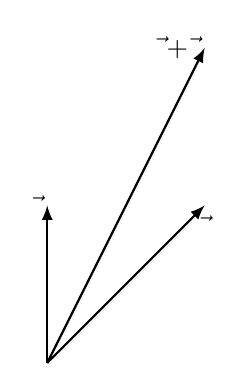
\begin{tikzpicture}
        \draw[thick,-latex] (0,0) -- (0,2) node[left]{$\vec{\x}$};
        \draw[thick,-latex] (0,0) -- (2,4) node[left]{$\vec{\x}+ \vec{\y}$};
        \draw[thick,-latex] (0,0) -- (2,2) node[below]{$\vec{\y}$};
    \end{tikzpicture}
    }
    \subfigure[多项式]{
    \begin{tikzpicture}
        \begin{axis}[xlabel=$x$, ylabel=$y$, domain=-2.5:2.5]
        \addplot[color=red]{-2 * x ^ 2};
        \addplot[color=blue] {-3*x + 3};
        \addplot[color=orange] {(x-2) ^ 2 - 5};
        \end{axis}
    \end{tikzpicture}
    }
    \caption{不同类型的向量。 向量令人惊讶, 包括(a)几何向量和(b)多项式}
    \end{figure}

    \item 音频信号(audio signals)是向量。
    音频信号表示为一系列数字。
    我们可以将两个音频信号相加, 和是一个新的音频信号。
    如果我们缩放(scale)音频信号, 我们也获取一段音频信号。
    因此, 音频信号也是一种向量。

    \item $\R^n$(n个实数的元组) 的元素是向量。
    $\R^n$ 比多项式更抽象, 也是这本书我们关注的重点。 例如:
    \begin{equation}
        \a =
        \begin{bmatrix}
            1 \\ 2 \\ 3
        \end{bmatrix}
        \in \R^3
    \end{equation}
    是一个数字三元组的例子。
    两个向量$\a , \b \in \R^n$ 相加,
    结果是另一个向量$\a + \b = \bs{c} \in \R^n$。
    更进一步, 用$\lambda \in \R$ 乘以 $\a \in \R^n$,
    结果是一个缩放的向量 $\lambda \a \in \R^n$。
    \marginpar{在计算机上实现时, 一定要注意检查数组操作是否真的是一个向量运算}
    将向量看作$\R^n$的元素有额外的好处, 他们松散对应着计算机上的实数数组
    许多编程语言支持数组操作,允许涉及向量运算的算法的便捷实现。
\end{enumerate}

线性代数关注向量概念间的相似性
线性代数侧重于这些向量概念之间的相似性。
我们可以将它们加在一起并乘以标量。
我们将在很大程度上关注 $\R^n$ 中的向量,因为线性代数中的大多数算法都在 $\R^n$ 中制定。
我们将在第 8 章中看到,我们经常将数据视为表示为 $\R^n$ 中的向量。
在本书中,我们将重点关注有限维向量空间,这种情况下在任何类型的向量和 $\R^n$ 之间存在 1:1 的对应关系。
方便的时候我们会用关于几何向量的直觉并考虑基于数组的算法。

数学中的一个主要思想是“闭包”的思想。
这是问题:我提议的操作可能产生的所有事物的集合是什么?
在向量的情况下:从一小组向量开始,然后将它们相加并缩放它们可以得到的向量集是什么?
结果就是向量空间(第 2.4 节)。
向量空间的概念及其属性是机器学习中非常底层的东西。
本章介绍的概念总结在图 2.2 中。

本章主要基于 Drumm和 Weil (2001)、Strang (2003)、Hogben (2013)、Liesen 和 Mehrmann (2015) 的讲义和书籍,以及 Pavel Grinfeld 的线性代数系列。
其他精彩的资源: MIT Gilbert Strang的线性代数课程和3BlueBrown的线性代数系列
\marginpar{
    \tiny{
    Pavel Grinfeld的系列线性代数课: \url{http://tinyurl.com/nahclwm}\\
    Gilber Strang's线性代数课: \url{http://tinyurl.com/29p5q8j}\\
    3BlueBrown线性代数系列课: \url{https://tinyurl.com/h5g4kps}
    }
}

\begin{figure}
    \begin{tikzpicture}[scale=0.4, align=center,rounded corners]
        \fontsize{8}{3}
        \node[fill=blue!20](Vector) at (0,0) {向量};
        \node[fill=blue!20](Matrix) at (-5,-5) {矩阵};
        \node[fill=blue!20](Vector space) at (0, -6) {向量空间};
        \node[fill=blue!20](Group) at (10, -6) {群};
        \node[fill=blue!20](Linear independence) at (17, -6) {线性\\无关};
        \node[fill=blue!20](Basis) at (17, -13) {基};
        \node[fill=blue!20](System of linear equations) at (-12, -10) {线性\\方程组};
        \node[fill=blue!20](Gaussian elimination) at (-12, -17) {高斯\\消元法};
        \node[fill=blue!20](Matrix inverse) at ( -5, -16) {逆矩阵};
        \node[fill=blue!20](Linear/affine mapping) at ( -2, -12) {线性/仿射映射};

        \node[fill=green!20](Chapter3) at (-2, -20) {Chapter3\\解析几何};
        \node[fill=green!20](Chapter5) at (-15, -5) {Chapter5\\向量积分};
        \node[fill=green!20](Chapter10) at (17, -20) {Chapter10\\降维};
        \node[fill=green!20](Chapter12) at (10, -20) {Chapter12\\分类};

        \draw[-latex] (Vector) -- node[above left]{组合} (Matrix);
        \draw[-latex] (Matrix) -- node[above left]{表示} (System of linear equations);
        \draw[-latex] (Matrix) -- node[above left]{表示} (Linear/affine mapping);
        \draw[-latex] (Matrix) --  (Chapter5);
        \draw[-latex] (System of linear equations) -- node[above left]{被解决}(Gaussian elimination);
        \draw[-latex] (System of linear equations) -- node[above right]{解决} (Matrix inverse);

        \draw[-latex] (Vector) -- node[above right]{闭包} (Vector space);
        \draw[-latex] (Vector space) -- (Linear/affine mapping);
        \draw[-latex] (Linear/affine mapping) -- (Chapter3);
        \draw[-latex] (Linear/affine mapping) -- (Chapter12);

        \draw[-latex] (Group) -- node[above]{阿贝尔\\with +} (Vector space);

        \draw[-latex] (Vector) -- node[above right]{的属性}(Linear independence);
        \draw[-latex] (Linear independence) -- node[above right]{最大集} (Basis);
        \draw[-latex] (Basis) -- (Chapter10);
        \draw[-latex] (Basis) -- (Chapter12);
    \end{tikzpicture}
    \caption{本章概念的思维导图, 以及本书其他部分使用它们的地}
\end{figure}

线性代数在机器学习和通用数学中扮演着重要的角色。
本章介绍的概念进一步扩展到第 3 章中的几何概念。
在第 5 章中,我们将讨论向量微积分,其中矩阵运算的基本知识是必不可少的。
在第 10 章中,我们将使用投影(将在第 3.8 节中介绍)通过主成分分析(PCA)进行降维。
在第 9 章中,我们将讨论线性回归,线性代数在解决最小二乘问题中起着核心作用。

\section{线性方程组}

线性方程组是线性代数的核心部分。
许多问题可以表述为线性方程组,而线性代数为我们提供了解决它们的工具。

\begin{example}
    一家公司生产产品 $N_1,...,N_n$, 需要资源$R_1 ,..., R_m$。
    生产一单位产品 $N_j$, 需要$a_{ij}$单位资源$R_i$,
    其中 $i = 1,..., m$ 和 $j = 1,...,n$.
    
    目标是找到一个最优的生产计划,i.e.,
    如果总共有 $b_i$ 个单位的资源$R_i$可用,则应该生产多少单位$x_j$的产品 $N_j$,
    并且(理想情况下)没有剩余资源。
    
    如果我们生产$x_1, ..., x_n$单位对应的产品, 我们总计需要
    \begin{equation}
        a_{i1}x_1 + ... + a_{in}x_n
    \end{equation}
    单位的资源$R_i$.
    一份优化的产品计划$(x_1, ..., x_n) \in \R^n$, 因此, 满足下面的方程组:
    \begin{equation}
    \begin{aligned}
            \begin{array}{rl}
                a_{11}x_1 + ... + a_{1n}x_n &= b_1 \\
                \vdots\\
                a_{m1}x_1 + ... + a_{mn}x_n &= b_m
            \end{array}
    \end{aligned}
    \end{equation}
    这里$a_{ij} \in \R$ and $b_i \in \R$.
\end{example}

方程 (2.3) 是线性方程组\marginpar{线性方程组}的一般形式,并且$x_1,..., x_n$ 是这个方程的未知数。
满足(2.3)的每一个n元组$(x_1,\dots, x_n ) \in \R^n$都是线性方程组的一个解\marginpar{解}。

\begin{example}
    线性方程组
    \begin{equation}
        \begin{aligned}
            x_1 & + x_2 & + &x_3 &= 3 \qquad (1)\\
             x_1 & - x_2 & + & 2x_3 &= 2 \qquad (2) \\
            2x_1 & & + &3x_3 &= 1 \qquad (3) \\
        \end{aligned}
    \end{equation}
    无解: 将前两个等式相加得到$2x_1 + 3x_3 = 5$, 这与等式$(3)$矛盾。

    我们再来看看线性方程组
    \begin{equation}
        \begin{aligned}
            x_1 & + & x_2 & + &x_3 &= 3 \qquad (1)\\
            x_1 & - & x_2 & + &2x_3 &= 2 \qquad (2) \\
                 &   & x_2 & + &x_3 &= 2 \qquad (3) \\
        \end{aligned}
    \end{equation}
    从等式(1)和(3), 可以推出$x_1 = 1$.
    从(1) + (2), 我们得到 $2x_1 + 3x_3 = 5$, i.e., $x_3 = 1$.
    从(3), 我们得到 $x_2 = 1$ .
    因此, $(1,1,1)$ 是可能的且唯一的解(可以通过带入方程验证一下).

    第三个例子, 我们思考
    \begin{equation}
        \begin{aligned}
            x_1 & + & x_2 & + &x_3 &= 3 \qquad (1)\\
            x_1 & - & x_2 & + &2x_3 &= 2 \qquad (2) \\
            2x_2&   &     & + &x_3 &= 5 \qquad (3) \\
        \end{aligned}
    \end{equation}
    因为(1) + (2) = (3), 我们可以忽略第三个等式(冗余的).
    从(1)和(2), 我们得到$2x_1 = 5 - 3x_3$ 和 $2x_2 = 1 + x_3$.
    我们定义只有变量$x_3 = a \in \R$, 使得任意三元组
    \begin{equation}
        \left(
        \frac{5}{2} - \frac{3}{2}a, \frac{1}{2} + \frac{1}{2} a, a
        \right),
        a \in \R
    \end{equation}
    都是该线性方程组的解, i.e., 我们得到一个包含无限多个解的解集。
\end{example}

\begin{figure}
    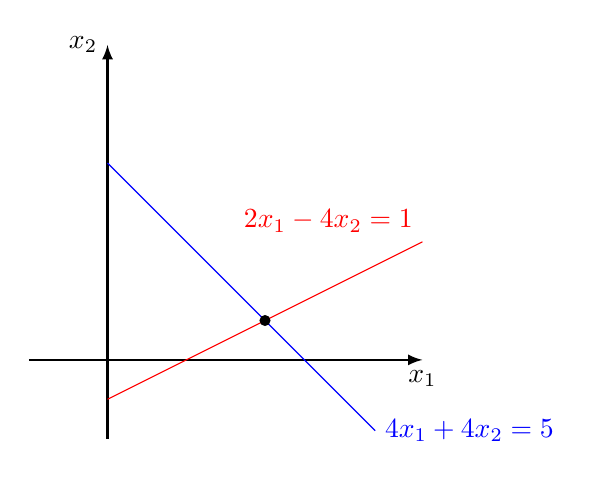
\begin{tikzpicture}[scale=2]
        \draw[thick, -latex] (0,-0.5) -- (0,2) node[left] {$x_2$};
        \draw[thick, -latex] (-0.5,0) -- (2,0) node[below] {$x_1$};

        \draw[color=red ,domain=0:2]plot(\x,{((1/2)*\x)-0.25})
        node[above left]{$2x_1 - 4x_2 = 1$};
        \draw[color=blue ,domain=0:1.7] plot(\x,{5/4 - (\x)}) node[right]{$4x_1 + 4x_2 = 5$};
        \fill (1,0.25) circle[radius=1pt];
    \end{tikzpicture}
    \caption{具有两个变量的两个线性方程的方程组的解空间(solution space)可以在几何上解释为两条线的交点。 每个线性方程代表一条线。}
\end{figure}

一般而言,对于实值线性方程组,我们要么没有,要么只有一个,要么有无穷多个解。
当我们无法求解线性方程组时,线性回归(第 9 章)解决了例2.1 的一个版本。

\begin{remark}[线性方程组的几何解释].
在具有两个变量 $x_1,x_2$ 的线性方程组中,每个线性方程定义 $x_1x_2$ 平面上的一条线。
由于线性方程组的解必须同时满足所有方程,因此解集是这些线的交点。
该交集可以是一条线(如果线性方程描述同一条线)、一个点或空集(当这些线平行时)。
图 2.3 给出了说明

\begin{equation}
    \begin{aligned}
        4x_1 + 4x_2 = 5\\
        2x_1 + 4x_2 = 1
    \end{aligned}
\end{equation}

其中解空间是点 $(x_1, x_2) = (1, \frac{1}{4})$。
类似地,对于三个变量,每个线性方程确定三维空间中的一个平面。
当我们将平面相交时,即同时满足所有线性方程,我们可以得到一个解集,它是一个平面、一条线、一个点或空集(当这些平面没有公共交集时)。
\hfill$\lozenge$
\end{remark}

对于求解线性方程组的系统方法,我们将引入一个有用的紧凑符号。
我们将系数 $a_{ij}$ 收集到向量中并将向量集中到矩阵中。
换句话说,我们按照以下形式编写(2.3)中的方程组:

\begin{align}
\begin{bmatrix}
    a_{11} \\ \vdots \\    a_{m1}
\end{bmatrix}
x_1 +
\begin{bmatrix}
    a_{12} \\ \vdots \\    a_{m2}
\end{bmatrix}
x_2 + \dots
\begin{bmatrix}
    a_{1n} \\ \vdots \\    a_{mn}
\end{bmatrix}
x_n =
\begin{bmatrix}
    b_1 \\ \vdots \\ b_m
\end{bmatrix}\\
\Longleftrightarrow
\begin{bmatrix}
    a_{11} & \dots & a_{1n} \\
    \vdots & &\vdots  \\
    a_{m1} & \dots & a_{mn} \\
\end{bmatrix}
\begin{bmatrix}
    x_1 \\ \vdots \\ x_n
\end{bmatrix}
=
\begin{bmatrix}
    b_1 \\ \vdots \\ b_m
\end{bmatrix}.
\end{align}

下面,我们将仔细研究这些矩阵并定义计算规则。
我们将在 2.3 节返回求解线性方程。

\section{矩阵}

矩阵在线性代数中起着核心作用。
它们可用于紧凑地表示线性方程组,但它们也表示线性函数(线性映射),我们将在后面的 2.7 节中看到。
在我们讨论这些有趣的话题之前,让我们首先定义矩阵是什么以及我们可以对矩阵进行什么样的操作。
我们将在第 4 章看到更多矩阵的性质。

\begin{definition}[矩阵].
    \marginpar{矩阵}
    对于 $m, n \in \mb{N}$的实值 $(m, n)$ 矩阵 $\A$
    是由元素 $a_{ij}$ 组成的 $m \cdot n$-元组,
    其中$i = 1, \dots, m$, $j = 1,\dots, n$,
    并根据m行和n列的矩形排列:

    \begin{equation}
        \A =
        \begin{bmatrix}
            a_{11} & a_{12} & \dots & a_{1n} \\
            a_{21} & a_{22} & \dots & a_{2n} \\
            \vdots & \vdots &       & \vdots \\
            a_{m1} & a_{m2} & \dots & a_{mn}
        \end{bmatrix},
        a_{ij} \in \R.
    \end{equation}
\end{definition}
按照惯例,$(1, n)$-矩阵称为行\marginpar{行},$(m, 1)$-矩阵称为列\marginpar{列}。
这些特殊矩阵也称为行/列向量\marginpar{行向量}\marginpar{列向量}。

$\R^{m \times n}$ 是所有实值$(m, n)$矩阵的集合。
$\A \in \R^{m \times n}$可以通过
将矩阵的所有$n$列堆叠成一个长向量来等价表示为
$\a \in \R^{mn}$;见图 2.4.

\begin{figure}[H]
    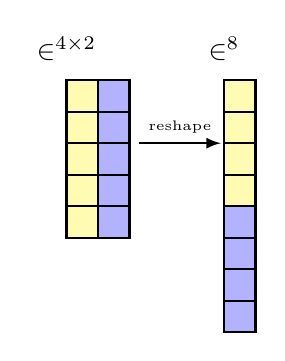
\begin{tikzpicture}[scale=0.4]
        \foreach \i in {0,-1, -2, -3, -4} {
        \filldraw[thick,fill=yellow!30,draw=black] (0,\i) rectangle (1,\i-1);
        \filldraw[thick,fill=blue!30,draw=black] (1,\i) rectangle (2,\i-1);
        }
        \foreach \i in {0,-1, -2, -3} {
        \filldraw[thick,fill=yellow!30,draw=black] (5,\i) rectangle (6,\i-1);
        }
        \foreach \i in {-4, -5,-6, -7} {
            \filldraw[thick,fill=blue!30,draw=black] (5,\i) rectangle (6,\i-1);
        }
        \draw[thick, -latex] (2.3,-2) -- node[above]{\tiny{reshape}}(4.9, -2);
        \node at (0,1) {$\A \in \R^{4 \times 2}$};
        \node at (5,1) {$\A \in \R^8$};
    \end{tikzpicture}
    \caption{通过堆叠列, 矩阵$\A$\\能够表示为一个长向量$\A$}
\end{figure}

注意矩阵的大小
\begin{verbatim}
    C = np.einsum(’il, lj’, A, B);
\end{verbatim}

\subsection{矩阵加法和乘法}

两个矩阵
$\A \in \R^{m \times n}$, $\B \in \R^{m \times n}$的和定义为逐元素的和。 i.e.,

\begin{equation}
    \A + \B :=
    \begin{bmatrix}
        a_{11} + b_{11} & \dots & a_{1n} + b_{1n} \\
        \vdots          &       & \vdots \\
        a_{m1} + b_{m1} & \dots & a_{mn} + b_{mn} \\
    \end{bmatrix}
    \in \R^{m \times n}
\end{equation}

对于矩阵
$\A \in \R^{m \times n}$,
$\B \in \R^{n \times k}$,
$\bs{C} = \A\B \in \R^{m \times k}$
的元素$c_{ij}$计算为

\begin{equation}
    c_{ij} = \sum_{l=1}^{n}a_{il}b_{lj},\quad i = 1, ..., m, \quad j = 1, ...,k.
\end{equation}

\marginpar{
    $\A$ 中有 n 列,$\B$ 中有 n 行,
    因此我们可以计算$a_{il}b_{lj}$,其中 $l = 1,...n$.
    通常,两个向量 $\a, \b$ 之间的点积表示为 $\a^\top\b$ 或$\langle \a, \b \rangle$.
}

这意味着,为了计算元素 $c_{ij}$,
我们将 $\A$ 的第 i 行的元素与 $\B$ 的第 j 列的元素相乘,然后将它们相加。
稍后在第 3.2 节中,我们将称其为相应行和列的点积。
在需要明确表示正在执行乘法的情况下,我们使用符号 $\A \cdot \A$ 来表示乘法(明确显示“$\cdot$”)。

\begin{remark}
    只有当两个矩阵的“相邻”维度匹配时,矩阵才能相乘。
    例如,一个 $n \times k$ 矩阵 $\A$ 可以与一个 $k \times m$ 矩阵 $\B$ 相乘,但只能从左侧开始:
    \begin{equation}
        \underbrace{\A}_{n \times k}
        \underbrace{\B}_{k \times m}=
        \underbrace{\bs{C}}_{n \times m}
    \end{equation}
    如果$ m \neq n$, 积$\B\A$未定义, 因为相邻维度不匹配。
    \hfill$\lozenge$
\end{remark}

\begin{remark}
    矩阵乘法并未定义为对矩阵元素的逐元素运算,
    即 $c_{ij} \neq a_{ij} b_{ij}$
    (即使$\A、\B$的大小选择适当)。
    我们将(多维)数组彼此相乘,这种逐元素乘法经常出现在编程语言中,称为哈达玛(Hadamard)乘积。
    \marginpar{哈达玛乘积}
    \hfill$\lozenge$
\end{remark}

\begin{example}
    对于
    $
    \A =
    \begin{bmatrix}
        1 & 2 & 3 \\
        3 & 2 & 1
    \end{bmatrix}
    \in \R^{2 \times 3},
    \B =
    \begin{bmatrix}
        0 & 2 \\
        1 & -1 \\
        0 & 1
    \end{bmatrix}
    \in \R^{3 \times 2}
    $,
    我们可得
    \begin{equation}
        \A\B =
        \begin{bmatrix}
            1 & 2 & 3 \\
            3 & 2 & 1
        \end{bmatrix}
        \begin{bmatrix}
            0 & 2 \\
            1 & -1 \\
            0 & 1 \\
        \end{bmatrix}
        =
        \begin{bmatrix}
            2 & 3 \\
            2 & 5
        \end{bmatrix}
        \in \R^{2 \times 2},
    \end{equation}
    \begin{equation}
        \B\A =
        \begin{bmatrix}
            0 & 2 \\
            1 & -1 \\
            0 & 1
        \end{bmatrix}
        \begin{bmatrix}
            1 & 2 & 3 \\
            3 & 2 & 1
        \end{bmatrix}
        =
        \begin{bmatrix}
            6 & 4 & 2 \\
            -2 & 0 & 2 \\
            3 & 2 & 1
        \end{bmatrix}
        \in \R^{3 \times 3}.
    \end{equation}
\end{example}

在这个例子中, 我们已经看到矩阵乘法并不符合交换律(is not commutative), i.e.,
$\A\B \neq \B\A$
另请参见图 2.5 中的说明。

\begin{figure}
    \caption{
        即便矩阵的积$\A\B$和$\B\A$有定义,
        他们结果也是不同的。
    }
    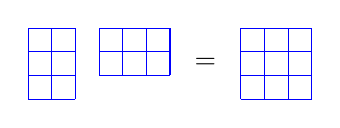
\begin{tikzpicture}[scale=0.3]
        \draw[draw=blue,step=1] (0,0) grid (2,-3);
        \draw[draw=blue,step=1] (3,0) grid (6,-2);
        \node at (7.5,-1.5) {$=$};
        \draw[draw=blue,step=1] (9,0) grid (12,-3);
    \end{tikzpicture}\\\\
    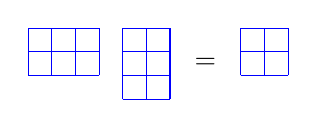
\begin{tikzpicture}[scale=0.3]
        \draw[draw=blue,step=1] (0,0) grid (3,-2);
        \draw[draw=blue,step=1] (4,0) grid (6,-3);
        \node at (7.5,-1.5) {$=$};
        \draw[draw=blue,step=1] (9,0) grid (11,-2);
\end{tikzpicture}
\end{figure}

\begin{definition}[单位矩阵(identity matrix)].
    在$\R^{n \times n}$,我们定义单位矩阵为对角线上都是1, 其余都是0的$n \times n$-矩阵。
    \begin{equation}
        \bs{I}_n :=
        \begin{bmatrix}
            1 & 0 & \dots & 0 & \dots & 0 \\
            0 & 1 & \dots & 0 & \dots & 0 \\
            \vdots & \vdots & \ddots & \vdots & \ddots & \vdots \\
            0 & 0 & \dots & 1 & \dots & 0 \\
            \vdots & \vdots & \ddots & \vdots & \ddots & \vdots \\
            0 & 0 & \dots & 0 & \dots & 1 \\
        \end{bmatrix}
        \in \R^{n \times n}
    \end{equation}
\end{definition}

现在我们已经定义了矩阵乘法, 矩阵加法和单位矩阵, 让我们来看一些矩阵的属性:

\begin{itemize}
    \item 结合律(Associativity):\marginpar{结合律}
    \begin{equation}
        \forall
        \A \in \R^{m \times n},
        \B \in \R^{n \times p},
        \bs{C} \in \R^{p \times q}:
        (\A\B)\bs{C} = \A(\B\bs{C})
    \end{equation}
    \item 分配律(Distrubutivity):\marginpar{分配律}
    \begin{subequations}
    \begin{align}
        \forall
        \A,\B \in \R^{m \times n},
        \bs{C},\bs{D} \in \R^{n \times p}:
        (\A + \B)\bs{C}=
        \A\bs{C} + \B\bs{C} \\
        \A(\bs{C} + \bs{D})=
        \A\bs{C} + \A\bs{D}
    \end{align}
    \end{subequations}
    \item 与单位矩阵相乘(Multiplication with the identity matrxi)
    \begin{equation}
        \forall \A \in \R^{m \times n}:
        \bs{I}_m\A=
        \A\bs{I}_n = \A
    \end{equation}
    注意如果 $m \neq n$, $\bs{I}_m \neq \bs{I}_n$
\end{itemize}

\subsection{逆矩阵和转置(inverse and transpose)}

\begin{definition}[逆(Inverse)].
    考虑一个方阵(squar matrix)
    \marginpar{ 方阵具有相同的行数和列数 }
    $\A \in \R^{n \times n}$。
    让矩阵$\B \in \R^{n \times n}$
    具有 $\A\B = \bs{I}_n = \B\A$ 的性质。
    $\B$ 被称为 $\A$ 的逆(矩阵)\marginpar{逆(矩阵)},用 $\A^{−1}$ 表示。
\end{definition}

不幸的是,并非每个矩阵 $\A$ 都具有逆 $\A^{-1}$.
如果这逆确实存在,$\A$ 称为常规/可逆/非奇异的\marginpar{常规/可逆/非奇异},
否则称为奇异/不可逆的。\marginpar{奇异/不可逆}
当逆矩阵存在时,它是唯一的。
在 2.3 节中,我们将讨论通过求解线性方程组来计算矩阵逆的一般方法。

\begin{remark}
    $2 \times 2$-矩阵的逆的存在性。 考虑如下矩阵
    \begin{equation}
        \A :=
        \begin{bmatrix}
            a_{11} & a_{12} \\
            a_{21} & a_{22}
        \end{bmatrix}
        \in \R^{2 \times 2}
    \end{equation}
    如果我们给$\A$乘以
    \begin{equation}
        \A' :=
        \begin{bmatrix}
            a_{22} & - a_{12} \\
            - a_{21} & a_{11}
        \end{bmatrix}
    \end{equation}
    我们得到
    \begin{equation}
        \A\A' =
        \begin{bmatrix}
            a_{11}a_{22} - a_{12}a_{21} & 0 \\
            0 & a_{11}a_{22} - a_{12}a_{21}
        \end{bmatrix}=
        (a_{11}a_{22} - a_{12}a_{21}) \bs{I}.
    \end{equation}
    因此,
    \begin{equation}
        \A' =
        \frac{1}{a_{11}a_{22} - a_{12}a_{21}}
        \begin{bmatrix}
            a_{22} & - a_{12} \\
            - a_{21} & a_{11}
        \end{bmatrix}
    \end{equation}
    当且仅当$a_{11}a_{22} - a_{12}a_{21} \neq 0$.
    在4.1节中, 我们会看到$a_{11}a_{22} - a_{12}a_{21}$是$2 \times 2$-矩阵的行列式(determinant).
    此外,我们可以使用行列式检查矩阵是否可逆。\hfill $\lozenge$
\end{remark}

\begin{example}[逆矩阵].\\
    矩阵
    \begin{equation}
        \A=
        \begin{bmatrix}
            1 & 2 & 1 \\
            4 & 4 & 5 \\
            6 & 7 & 7
        \end{bmatrix},
        \B=
        \begin{bmatrix}
            -7 & -7 & 6 \\
            2 & 1 & -1 \\
            4 & 5 & -4
        \end{bmatrix}
    \end{equation}
    互逆, 因为$\A\B = \bs{I} = \B\A$
\end{example}

\begin{definition}[转置(transpose)].
    \marginpar{转置}
    对于$\A \in \R^{m \times n}$,
    矩阵$\B \in \R^{n \times m}$称作矩阵$\A$的转置,
    其中$b_{ij} = a_{ji}$.
    我们写作$\B = \A^\top$.
\end{definition}
\marginpar{
矩阵$\A$的主对角线\\(main diagonal)
(有时称为"principal diagonal", "primary diagonal",or "major diagonal")
是条目 $a_{ij}$ 的集合,其中 $i = j$.
}

一般来说, 我们可以通过将$\A$的列写作$\A$的行得到$\A^\top$.
下面是关于逆矩阵和转置的重要性质:
\begin{align}
    \A\A^{-1} &= \bs{I} = \A^{-1}\A \\
    (\A\B)^{-1} &= \B^{-1} \A^{-1} \\
    (\A + \B)^{-1} &\neq \A^{-1}\B^{-1} \\
    (\A^\top)^\top &= \A \\
    (\A + \B) ^ \top &= \A^\top + \B ^ \top \\
    (\A\B)^\top &= \B^\top \A ^ \top
\end{align}
\marginpar{
    (2.28)的标量例子是
    \[ \frac{1}{2+4} = \frac{1}{6} \neq \frac{1}{2} + \frac{1}{4} \]
}

\begin{definition}[对称矩阵(symmetric matrix)].
    \marginpar{对称矩阵}
    矩阵$\A \in \R^{n \times n}$ 是对称的,
    如果$\A = \A ^ \top$
\end{definition}

请注意,只有 $(n, n)$-矩阵可以是对称的。
通常,我们将 $(n, n)$-矩阵也称为方阵\marginpar{方阵},因为它们具有相同的行数和列数。
此外,如果 $\A$ 是可逆的,那么 $\A^\top$ 也是可逆的,
并且 $(\A^{−1})^\top = (\A^\top)^{−1} =: \A^{-\top}$.

\begin{remark}[对称矩阵的和与积]
    对称矩阵$\A,\B \in \R^{n \times n}$的和总是对称的。
    但是, 尽管它们的积有定义, 却通常不是对称的:
    \begin{equation}
        \begin{bmatrix}
            1 & 0 \\
            0 & 0
        \end{bmatrix}
        \begin{bmatrix}
            1 & 1 \\
            1 & 1
        \end{bmatrix}
        =
        \begin{bmatrix}
            1 & 1 \\
            0 & 0
        \end{bmatrix}
    \end{equation}
    \hfill $\lozenge$
\end{remark}

\subsection{乘以标量(标量乘法)}

让我们看看当矩阵乘以标量 $\lambda \in \R$ 时会发生什么。
令 $\A \in \R^{m \times n}$ 并且 $\lambda \in \R$.
然后 $\lambda\A = \bs{K}$, $K_{ij} = \lambda a_{ij}$.
实际上,$\lambda$ 乘以$\A$的每个元素。
对于 $\lambda, \psi \in \R$,以下成立:

\begin{itemize}
    \item 结合律:\marginpar{结合律}\\ $(\lambda\psi)\bs{C} = \lambda(\psi\bs{C}), \quad \bs{C} \in \R ^{m \times n}$
    \item
    $
    \lambda (\B\bs{C}) =
    (\lambda\B) \bs{C} =
    \B(\lambda \bs{C}) =
    (\B\bs{C}) \lambda,
    \quad
    \B \in \R^{m \times n},
    \bs{C} \in \R^{n \times k}
    $.
    \item
    $
    (\lambda \bs{C})^\top =
    \bs{C}^\top \lambda^\top =
    \bs{C}^\top \lambda =
    \lambda \bs{C}^\top
    $, 因为对于所有的$\lambda \in \R$, 有$\lambda = \lambda^\top$
    \item 分配律:\marginpar{分配律}\\
    $
    (\lambda + \psi) \bs{C} = \lambda \bs{C} + \psi \bs{C},\quad \bs{C} \in \R^{m \times n}\\
    \lambda(\B + \bs{C}) = \lambda \B + \lambda \bs{C}, \quad \B, \bs{C} \in \R^{m \times n}
    $
\end{itemize}

\begin{example}
    \textbf{分配律}\\
    如果我们定义
    \begin{equation}
        \bs{C} :=
        \begin{bmatrix}
            1 & 2 \\
            3 & 4
        \end{bmatrix},
    \end{equation}
    那么对于任意$\lambda, \psi \in \R$, 我们有
    \begin{subequations}
        \begin{align}
            (\lambda + \psi) \bs{C} &=
            \begin{bmatrix}
                (\lambda + \psi)1 & (\lambda + \psi)2 \\
                (\lambda + \psi)3 & (\lambda + \psi)4
            \end{bmatrix}
            =
            \begin{bmatrix}
                \lambda + \psi & 2\lambda + 2\psi \\
                3\lambda + 3\psi & 4\lambda + 4\psi
            \end{bmatrix}
            \\&=
            \begin{bmatrix}
                \lambda & 2\lambda \\
                3\lambda & 4\lambda
            \end{bmatrix}
            +
            \begin{bmatrix}
                \psi & 2\psi \\
                3\psi & 4\psi
            \end{bmatrix}
            =
            \lambda\bs{C} + \psi \bs{C}.
        \end{align}
    \end{subequations}
\end{example}

\subsection{线性方程组的简洁表示法}

我们考虑下面这个线性方程组:

\begin{equation}
    \begin{aligned}
        2x_1 + 3x_2 + 5x_3 = 1 \\
        4x_1 + 2x_2 - 7x_3 = 8 \\
        9x_1 + 5x_2 - 3x_3 = 2 \\
    \end{aligned}
\end{equation}

利用矩阵乘法的规则, 我们可以将这个线性方程组表达的更简洁

\begin{equation}
    \begin{bmatrix}
        2 & 3 & 5 \\
        4 & -2 & -7 \\
        9 & 5 & -3
    \end{bmatrix}
    \begin{bmatrix}
        x_1 \\ x_2 \\ x_3
    \end{bmatrix}
    =
    \begin{bmatrix}
        1 \\ 8 \\ 2
    \end{bmatrix}.
\end{equation}

注意$x_1$乘以第一列, $x_2$是第二列, $x_3$是第三列
\footnote{译者注:参考(2.9)(2.10), $\A$的每一列看作列向量}。

一般来说,一个线性方程组可以用它们的矩阵形式简洁地表示为
$\A\x = \b$;
见 (2.3),乘积 $\A\x$ 是 $\A$ 的列的(线性)组合。
我们将在 2.5 节中更详细地讨论线性组合。

\section{解线性方程组}

在(2.3), 我们介绍了方程组的一般形式, i.e.,

\begin{equation}
    \begin{aligned}
        a_{11}x_1 + \dots + a_{1n}x_n &= b_1 \\
        &\vdots\\
        a_{m1}x_1 + \dots + a_{mn}x_n &= b_m \\
    \end{aligned}
\end{equation}

其中, $a_{ij} \in \R$, $b_i \in \R$是已知常量,
$x_j$是未知数,$i=1,...,m$, $j=1,...,n$.

到目前为止,我们看到矩阵可以用作表示线性方程组的一种简洁方式,
因此我们可以写出 $\A\x = \b$,参见(2.10)。
此外,我们定义了基本的矩阵运算,例如矩阵的加法和乘法。
接下来,我们将专注于求解线性方程组,并提供用于求矩阵逆的算法。

\subsection{特解与通解}

在讨论如何对线性方程组求通解之前,让我们先看一个例子。
考虑方程组
\begin{equation}
    \begin{bmatrix}
        1 & 0 & 8 & -4 \\
        0 & 1 & 2 & 12
    \end{bmatrix}
    \begin{bmatrix}
        x_1 \\ x_2 \\ x_3 \\ x_4
    \end{bmatrix}
    =
    \begin{bmatrix}
        48 \\ 8
    \end{bmatrix}
\end{equation}
该方程组有两个方程和四个未知数。
因此,通常我们会期望有无穷多个解。
这个方程组的形式特别简单,其中前两列由 1 和 0 组成。
请记住,我们要找到标量 $x_1 , ..., x_4$,
使得 $\sum_{i=1}^{4} x_i \bs{c}_i = \b$
\footnote{
    译者注:参见式(2.9),(2.10), 可以将第一个矩阵的每一列视作列向量, 应用矩阵乘法规则, 即可得到该结果
},
其中我们定义 $\c_i$ 是矩阵的第$i$列,$\b$ 是(2.38)等号的右侧。
对第一列乘以42,第二列乘以8,可以立即得到 (2.38)的解
\begin{equation}
    \b =
    \begin{bmatrix}
        42 \\ 8
    \end{bmatrix}
    = 42
    \begin{bmatrix}
        1 \\ 0
    \end{bmatrix}
    +8
    \begin{bmatrix}
        0 \\ 1
    \end{bmatrix}
\end{equation}
因此,一个解是 $[42, 8, 0, 0]^\top$ 。
这个解称为特解(particular/special solutioin)。\marginpar{特殊解}
然而,这并不是这个线性方程组的唯一解。
为了获取所有其他解,我们需要以一种非平凡(non-trivial)
\footnote{
    译者注:
    在数学中,术语“平凡”通常用于指代具有非常简单结构的对象。
    "Trivial"也可用于描述结构非常简单的方程的解,但为完整起见不能省略。这些解称为平凡解。
    可以参考\url{https://en.wikipedia.org/wiki/Triviality_(mathematics)}
}
的方式生成 $\bs{0}$并创造性地使用矩阵的列:
给特解加上$\bs{0}$ 不会改变特解。
为此,我们使用前两列(这种非常简单的形式)表示第三列
\begin{equation}
    \begin{bmatrix} 8 \\ 2 \end{bmatrix}
    =8
    \begin{bmatrix} 1 \\ 0 \end{bmatrix}
    +2
    \begin{bmatrix} 0 \\ 1 \end{bmatrix}
\end{equation}
所以
$\bs{0}= 8\c_1 + 2\c_2 - 1\c_3 + 0\c_4$
并且$(x_2, x_2, x_3, x_4) = (8, 2, -1, 0)$.
事实上, $\lambda_1 \in \R$对该解的任何乘法都会生成$\bs{0}$向量,i.e.,
\begin{equation}
\begin{bmatrix}
    1 & 0 & 8 & -4 \\
    0 & 1 & 2 & 12
\end{bmatrix}
\left(
\lambda_1
\begin{bmatrix}
    8 \\ 2 \\ -1 \\ 0
\end{bmatrix}
\right)=
\lambda_1(8\bs{c}_1 + 2\bs{c}_2 - \bs{c}_3)
\end{equation}
按照相同的推理思路,我们使用前两列表示(2.38)中矩阵的第四列,并生成另一组非平凡版本的$\bs{0}$
\begin{equation}
    \begin{bmatrix}
        1 & 0 & 8 & -4 \\
        0 & 1 & 2 & 12
    \end{bmatrix}
    \left(
    \lambda_2
    \begin{bmatrix}
        -4 \\ 12 \\ 0 \\ -1
    \end{bmatrix}
    \right)
    =
    \lambda_2(-4\bs{c}_1 + 12\bs{c}_2 - \bs{c}_4)
\end{equation}
其中$\lambda_2 \in \R$.
综上所述,我们得到式(2.38)中方程组的所有解,称为通解(general solution),也就是解集:
\begin{equation}
    \left\{
    \x \in \R^4:
    \x=
    \begin{bmatrix} 42 \\ 8 \\ 0 \\ 0 \end{bmatrix}
    +\lambda_1
    \begin{bmatrix} 8 \\ 2 \\ -1 \\ 0 \end{bmatrix}
    +\lambda_2
    \begin{bmatrix} -4 \\ 12 \\ 0 \\ -1 \end{bmatrix}
    ,\lambda_1, \lambda_2 \in \R
    \right\}
\end{equation}

\begin{remark}
    我们遵循的一般方法包括以下三个步骤:
    \begin{enumerate}
        \item 找到 $\A\x = \b$ 的特定解。
        \item 找出 $\A\x = \bs{0}$ 的所有解。
        \item 将步骤 1. 和 2. 中的解合并为通解。
    \end{enumerate}
\end{remark}
一般或特殊的解决方案都不是唯一的。\hfill$\lozenge$

前面例子中的线性方程组很容易求解,
因为(2.38)中的矩阵具有这种特别方便的形式,
这使我们可以通过观察就能找到特解和通解。
然而,一般方程组不是这种简单的形式。
幸运的是,存在一种将任何线性方程组转换为这种特别简单的形式的建设性算法:高斯消元法。
高斯消元的关键是线性方程组的初等变换(elementary transformations),将方程组转化为简单的形式。
然后,我们可以将这三个步骤应用到我们刚刚在 (2.38) 示例的上下文中讨论的简单形式。

\subsection{初等变换}
\marginpar{初等变换}

求解线性方程组的关键是使用保持解集相同的初等变换,但将方程组转换为更简单的形式:
\begin{itemize}
    \item 交换两个方程的位置(矩阵中的行代表方程组中的方程)
    \item 给方程(行)乘以一个常数$\lambda \in \R \backslash \{0\}$
    \item 两个方程(行)相加
\end{itemize}

\begin{example}
    已知$a \in \R$, 我们寻找下面这个方程组的全部解:
    \begin{equation}
        \begin{array}{rcrcrcrcrcr}
            -2x_1 & + & 4x_2 & - & 2x_3 & - & x_4  & + & 4x_5 & = & -3 \\
            4x_1  & - & 8x_2 & + & 3x_3 & - & 3x_4 & + & x_5  & = & 2 \\
            x_1   & - & 2x_2 & + & x_3  & - & x_4  & + & x_5  & = & 0 \\
            x_1   & - & 2x_2 &   &      & - & 3x_4 & + & 4x_4 & = & a
        \end{array}
    \end{equation}
    我们首先将这个方程组转换为简洁的矩阵符号 $\A\x = \b$.
    我们不再明确提及变量 $\x$ 并构建增广矩阵(augmented matrix)\marginpar{增广矩阵}
    (形式为 $[\A | \b ]$ )
    \[
        \begin{bmatrix}
        \begin{array}{rrrrr|r}
            −2 & 4 & −2 & −1 & 4 & −3 \\
            4 & −8 & 3 & −3 & 1 &  2 \\
            1 & −2 & 1 & -1 & 1 & 0 \\
            1 & -2 & 0 & -3 & 4 & a
        \end{array}
        \end{bmatrix}
        \begin{array}{l}
            \text{和}R_3\text{交换}\\
            \\
            \text{和}R_1\text{交换}\\
            \\
        \end{array}
    \]
    \marginpar{
        增广矩阵$[\A|\b]$紧凑/简洁的表示了线性方程组$\A\x=\b$
    }
    这里,我们使用垂直线将(2.44)中的左侧和右侧分开。
    我们使用$\rightsquigarrow$来表示进行了初等变换。

    交换第1行和第2行得到
    \[
    \begin{bmatrix}
        \begin{array}{rrrrr|r}
            1 & −2 & 1 & -1 & 1 & 0 \\
            4 & −8 & 3 & −3 & 1 &  2 \\
            −2 & 4 & −2 & −1 & 4 & −3 \\
            1 & -2 & 0 & -3 & 4 & a
        \end{array}
    \end{bmatrix}
    \begin{array}{l}
        \\
        -4R_1\\
        +2R_1\\
        -2R_1\\
    \end{array}
    \]
    现在当我们应用指定的转换时(例如,从第 2 行中减去第 1 行四次), 我们得到:
    \[
    \begin{bmatrix}
        \begin{array}{rrrrr|r}
            1  & −2 &  1 & -1 &  1 &  0 \\
            0  &  0 & -1 &  1 & -3 &  2 \\
            0  &  0 &  0 & −3 &  6 & −3 \\
            0  &  0 & -1 & -2 &  3 &  a
        \end{array}
    \end{bmatrix}
    \begin{array}{l}
        \\\\\\
        -R_2-R_3\\
    \end{array}
    \]
    \[
    \rightsquigarrow
    \begin{bmatrix}
        \begin{array}{rrrrr|r}
            1  & −2 &  1 & -1 &  1 &  0 \\
            0  &  0 & -1 &  1 & -3 &  2 \\
            0  &  0 &  0 & −3 &  6 & −3 \\
            0  &  0 &  0 &  0 &  3 & a+1
        \end{array}
    \end{bmatrix}
    \begin{array}{l}
        \\
        \cdot (-1) \\
        \cdot (-\frac{1}{3})
    \end{array}\\
    \]
    \[
    \rightsquigarrow
    \begin{bmatrix}
        \begin{array}{rrrrr|r}
            1  & −2 &  1 & -1 &  1 &  0 \\
            0  &  0 &  1 & -1 &  3 & -2 \\
            0  &  0 &  0 &  1 & -2 &  1 \\
            0  &  0 &  0 &  0 &  0 & a+1
        \end{array}
    \end{bmatrix}
    \]
    这个(增广)矩阵是一种方便的形式,是行阶梯形矩阵(row-echelon form, REF)\marginpar{行阶梯形矩阵}。
    使用我们要求解的变量将这个简洁的符号表示恢复为原本的显式符号表示\footnote{译者注:即将矩阵转换为对应的线性方程组},我们得到
    \begin{equation}
        \begin{array}{rcrcrcrcrcr}
            x_1 & - & 2x_2 & + & x_3 & - & x_4 & + &  x_5 & = & 0 \\
                &   &      &   & x_3 & - & x_4 & + & 3x_5 & = & -2 \\
                &   &      &   &     & - & x_4 & - & 2x_5 & = & 1 \\
                &   &      &   &     &   &     &   &    0 & = & a+1
        \end{array}
    \end{equation}
    只有$a=-1$, 这个方程才有解。 一个特解是\marginpar{特解}
    \begin{equation}
        \begin{bmatrix}
            x_1 \\ x_2 \\ x_3 \\ x_4 \\ x_5
        \end{bmatrix}
        =
        \begin{bmatrix}
            2 \\ 0 \\ -1 \\ 1 \\ 0
        \end{bmatrix}
    \end{equation}
    通解\marginpar{通解}, 则是:
    \begin{equation}
        \left\{
        \x \in \R^5:
        \x =
        \begin{bmatrix}
            2 \\ 0 \\ -1 \\ 1 \\ 0
        \end{bmatrix}
        +
        \lambda_1
        \begin{bmatrix}
            2 \\ 1 \\ 0 \\ 0 \\ 0
        \end{bmatrix}
        +
        \lambda_2
        \begin{bmatrix}
            2 \\ 0 \\ -1 \\ 2 \\ 1
        \end{bmatrix},
        \lambda_1, \lambda_2 \in \R
        \right\}.
    \end{equation}
\end{example}

接下来,我们将详细介绍一种构造性的方法来获得线性方程组的特解和通解。

\begin{remark}[主元和阶梯结构(Pivots and Staircase Structure)].\marginpar{主元}
    行的前导系数(从左侧开始的第一个非零数)称为主元,并且始终严格地位于其上方行主元的右侧。
    因此,任何行阶梯形的方程组都具有“阶梯”结构。 \hfill $\lozenge$
\end{remark}

\begin{definition}[行阶梯形矩阵].
    一个矩阵是行阶梯形矩阵如果\marginpar{行阶梯形矩阵}
    \begin{itemize}
        \item 所有只包含零的行都在矩阵的底部;相应地,所有包含至少一个非零元素的行都位于仅包含零的行的上方。
        \item 仅查看非零行,左侧的第一个非零数字(也称为主元或前导系数)始终严格位于其上方行的主元右侧。
        \marginpar{主元或前导系数}
    \end{itemize}
\end{definition}

\begin{remark}[基础变量与自由变量]
    \marginpar{基础变量与自由变量}
    行阶梯形矩阵中与主元对应的变量称为基础变量(basic variables), 其他变量称为自由变量(free variables).
    例如, (2.45)中, $x_1, x_3, x_4$ 是基础变量, $x_2, x_5$是自由变量。 \hfill $\lozenge$
\end{remark}

\begin{remark}[求得特解]
    当我们需要确定特解时,行阶梯形矩阵使我们的生活更轻松。
    为此,我们使用主元列表示方程组的右侧,使得
    $\b = \sum_{i=1}^{P} \lambda_i \bs{p}_i$,
    其中 $\bs{p}_i , i = 1, ..., P$ 是主元列。
    如果我们从最右边的主元列开始并向左工作,则最容易确定 $\lambda_i$。
    在前面的例子中, 我们尝试寻找$\lambda_1, \lambda_2, \lambda_3$使得
    \begin{equation}
        \lambda_1
        \begin{bmatrix}
            1 \\ 0 \\ 0 \\ 0
        \end{bmatrix}+
        \lambda_2
        \begin{bmatrix}
            1 \\ 1 \\ 0 \\ 0
        \end{bmatrix}+
        \lambda_3
        \begin{bmatrix}
            -1 \\ -1 \\ 1 \\ 0
        \end{bmatrix}=
        \begin{bmatrix}
            0 \\ -2 \\ 1 \\ 0
        \end{bmatrix}
    \end{equation}
    从这里,我们相对直接地发现
    $\lambda_3 = 1, \lambda_2 = -1, \lambda_1 = 2$。
    当我们把所有东西放在一起时,我们一定不要忘记我们将系数隐式设置为 0 的非主元列。
    因此,我们得到 特解 $\x = [2, 0, -1, 1, 0]^\top$。\hfill$\lozenge$
\end{remark}

\begin{remark}
(简约行阶梯形矩阵)\marginpar{简约行阶梯形矩阵}
简化列阶梯形矩阵或简约行梯形式矩阵(reduced row echelon form, also: row-recuced echelon form),也称作行规范形矩阵(row canonical form). 一个方程组是这种矩阵, 如果
\begin{itemize}
    \item 它是行阶梯形
    \item 每个主元是1
    \item 主元是所在列唯一的非零元素
\end{itemize}
\hfill $\lozenge$
\end{remark}

简约行梯形矩阵将在后面的2.3.3 节发挥重要作用,因为它允许我们以直接的方式确定线性方程组的通解。

\begin{remark}[高斯消元法].
    高斯消元是一种算法,它执行基本变换以将线性方程组变为简约行梯形。\marginpar{高斯消元法}\hfill $\lozenge$
\end{remark}

\begin{example}[简约行阶梯形矩阵]
    验证以下矩阵是否是简约行梯形矩阵(主元以\textbf{粗体}显示):
    \begin{equation}
        \A =
        \begin{bmatrix}
            \bs{1} & 3 & 0 & 0 & 3 \\
            0 & 0 & \bs{1} & 0 & 9 \\
            0 & 0 & 0 & \bs{1} & -4
        \end{bmatrix}
    \end{equation}
\end{example}

找到 $\A\x = \0$解的关键思想是查看非主元列,我们需要将其表示为主元列的(线性)组合。
简约行阶梯形矩阵使这相对简单,我们根据非主元列左侧的主元列的加和或乘积来表示非主元列:
第二列是第一列的3倍(我们可以忽略第二列右侧的主元列)。
因此, 为了得到$\0$, 我们需要从3倍的第一列中减去第二列。
现在,我们看第五列,这是我们的第二个非主元列。
第五列可以表示为第一个主元列的 3 倍、第二个主元列的 9 倍和第三个主元列的 -4 倍。
我们需要跟踪主元列的索引并将其转换为第一列的 3 倍,第二列(非主元列)的 0 倍,第三列(我们的第二个主元列)的 9 倍 ,以及 -4 乘以第四列(即第三个主元列)。
然后我们需要减去第五列得到0.
最后我们还是在求解一个齐次方程组

总而言之,$\A\x = \bs{0}, x \in \R^5$ 的所有解由下式给出

\begin{equation}
    \left\{
    \x \in \R^5:
    \x = \lambda_1
    \begin{bmatrix}
        3 \\ -1 \\ 0 \\ 0 \\ 0
    \end{bmatrix} + \lambda_2
    \begin{bmatrix}
        3 \\ 0 \\ 9 \\ -4 \\ -1
    \end{bmatrix},
    \lambda_1, \lambda_2 \in \R
    \right\}.
\end{equation}

\subsection{负1技巧}

接下来, 我们介绍一个实用的技巧来读出齐次线性方程组$\A\x = \bs{0}$的解,
这里$\A \in \R^{k \times n}, \x \in \R^n$.

首先, 我们假设$\A$是一个没有任何只含0的行的简约行阶梯形矩阵, i.e.,

\begin{equation}
    \A =
    \begin{bmatrix}
        \begin{array}{cccccccccccccccc}
                 0 & \dots &      0 &   \bs{1} &   \ast & \dots &   \ast &      0 &   \ast & \dots &   \ast &      0 & \ast & \dots & \ast \\
            \vdots &       & \vdots &      0 &      0 & \dots &      0 &     \bs{1} &   \ast & \dots &   \ast & \vdots & \ast & \dots & \ast \\
            \vdots &       & \vdots & \vdots & \vdots &       & \vdots &      0 & \vdots &       & \vdots & \vdots & \vdots & & \vdots \\
            \vdots &       & \vdots & \vdots & \vdots &       & \vdots & \vdots & \vdots &       & \vdots &      0 & \vdots & & \vdots \\
                 0 & \dots &      0 &      0 &      0 & \dots &      0 &      0 &      0 & \dots &      0 &     \bs{1} & \ast & \dots & \ast \\
        \end{array}
    \end{bmatrix},
\end{equation}
其中$\ast$可以是任意实数,约束条件是每行的第一个非零条目必须为 1,并且相应列中的所有其他项目必须为 0 .
有主元(以粗体标记)的列$j_1, ...,j_k$ 是标准单位向量 $e_1 , ..., e_k \in \R^k$。
我们可以将这个矩阵扩展为 $n \times n$ 矩阵,通过添加 $n − k$ 行
\begin{equation}
    \begin{bmatrix}
        0 & \dots & 0 & -1 & 0 & \dots & 0 \\
    \end{bmatrix}
\end{equation}
使得增广矩阵 $\tilde{\A}$ 的对角线包含 1 或 -1。
然后,包含 -1 作为主元的 $\tilde{\A}$ 列是齐次方程$\A\x = \bs{0}$的解。
更准确地说,这些列构成了$\A\x = \bs{0}$的解空间的基(第 2.6.1 节),我们稍后将其称为核空间(kernel space)或零空间(null space)(见第 2.7.3 节)
\marginpar{kernel/null space}

\begin{example}[负1技巧]
    让我们回顾(2.49)中的矩阵, 它已经是REF了:
    \begin{equation}
        \A =
        \begin{bmatrix}
            1 & 3 & 0 & 0 & 3 \\
            0 & 0 & 1 & 0 & 9 \\
            0 & 0 & 0 & 0 & -4
        \end{bmatrix}
    \end{equation}
    现在我们通过在对角线上缺失主元的地方添加(2.52)形式的行将这个矩阵增广到$5 \times 5$-矩阵, 得到
    \begin{equation}
        \tilde{\A} =
        \begin{bmatrix}
            1 & 3 & 0 & 0 & 3 \\
            \color{blue} 0 & \color{blue} \bs{-1} & \color{blue} 0 & \color{blue} 0 & \color{blue} 0 \\
            0 & 0 & 1 & 0 & 9 \\
            0 & 0 & 0 & 1 & -4 \\
            \color{blue} 0 & \color{blue} 0 & \color{blue} 0 & \color{blue} 0 & \color{blue} \bs{-1} \\
        \end{bmatrix}
    \end{equation}
    从这个形式, 我们可以立即读出$\A\x=\bs{0}$的解,
    只要取出$\tilde{\A}$中对角线包含$-1$的列即可:
    \begin{equation}
        \left\{
            \x \in \R^5:
            \x = \lambda_1
            \begin{bmatrix}
                3 \\ -1 \\ 0 \\ 0 \\ 0
            \end{bmatrix}
            + \lambda_2
            \begin{bmatrix}
                3 \\ 0 \\ 9 \\ -4 \\ -1
            \end{bmatrix},
            \lambda_1, \lambda_2 \in \R
        \right\},
    \end{equation}
\end{example}

\begin{center} 计算逆矩阵 \end{center}

为了求逆矩阵$\A^{-1}, \A \in \R^{n \times n}$
我们需要找到一个矩阵$\bs{X}$满足$\bs{AX}=\bs{I}_n$.
然后就有$\bs{X} = \A^{-1}$.
我们可以将其联立写成线性方程组$\bs{AX}=\bs{I}_n$,
其中我们求解 $\bs{X} = [\x_1|\dots|\x_n]$.
我们使用增广矩阵符号来紧凑表示这组线性方程组,并得到
\begin{equation}
    \begin{bmatrix}
        \A | \bs{I}_n
    \end{bmatrix}
    \quad
    \rightsquigarrow \dots \rightsquigarrow
    \quad
    \begin{bmatrix}
        \bs{I}_n | \A^{-1}
    \end{bmatrix}
    \footnote{
        译者注: 初等变换的结果可以看作是与原方程组等价的(不改变解集),
        $[\A|\I_n]$对应方程组 $\A\bs{X} = \I_n$,
        $[\I_n|\A^{-1}]$对应方程组 $\I_n \bs{X} = \A^{-1}$.
        通过简单的矩阵乘法易得$\I_n\bs{X} = \bs{X} = \A^{-1}$.
    }
\end{equation}
这意味着,如果我们将增广方程组简化为行阶梯形式,我们可以读出方程组右侧的逆。
因此,确定矩阵的逆等效于求解线性方程组。

\begin{example}
    (通过高斯消元法求解逆矩阵)\\
    为了确定以下矩阵的逆:
    \begin{equation}
        \A =
        \begin{bmatrix}
            1 & 0 & 2 & 0 \\
            1 & 1 & 0 & 0 \\
            1 & 2 & 0 & 1 \\
            1 & 1 & 1 & 1 \\
        \end{bmatrix}
    \end{equation}
    我们写下增广矩阵
    \[
    \begin{bmatrix}
        \begin{array}{cccc|cccc}
            1 & 0 & 2 & 0 & 1 & 0 & 0 & 0 \\
            1 & 1 & 0 & 0 & 0 & 1 & 0 & 0 \\
            1 & 2 & 0 & 1 & 0 & 0 & 1 & 0 \\
            1 & 1 & 1 & 1 & 0 & 0 & 0 & 1 \\
        \end{array}
    \end{bmatrix}
    \]
    然后使用高斯消元法把它转换为行阶梯形矩阵
    \[
    \begin{bmatrix}
        \begin{array}{cccc|cccc}
            1 & 0 & 0 & 0 & -1 & 2 & -2 & 2 \\
            0 & 1 & 0 & 0 & 1 & -1 & 2 & -2 \\
            0 & 0 & 1 & 0 & 1 & -1 & 1 & -1 \\
            0 & 0 & 0 & 1 & -1 & 0 & -1 & 2 \\
        \end{array}
    \end{bmatrix},
    \]
    如此, 欲求得的逆便在右手边了:
    \begin{equation}
    \A^{-1} =
    \begin{bmatrix}
        -1 & 2 & -2 & 2 \\
        1 & -1 & 2 & -2 \\
        1 & -1 & 1 & -1 \\
        -1 & 0 & -1 & 2 \\
    \end{bmatrix}.
    \end{equation}
    我们可以确认(2.58)就是所需的逆, 只要计算$\bs{AA}^{-1}$
    然后观察我们是否又得到了$\bs{I}_4$
\end{example}

\subsection{求解线性方程组的算法}

下面,我们简要讨论求解 $\A\x = \b$形式的线性方程组的方法。
我们假设存在一个解。
如果没有解,我们需要求助于近似解,本章不涉及。
解决近似问题的一种方法是使用线性回归方法,我们将在第 9 章详细讨论。

在特殊情况下,我们可能能够确定逆 $\A^{−1}$,
使得 $\A\x = \b$ 的解为 $\x = \A^{−1} \b$。
然而,这只有在$\A$是方阵且可逆时才有可能,但通常情况并非如此。
此外,在温和的假设(mild assumptions)下(即 $\A$ 需要具有线性无关的列),我们可以使用以下变换
\begin{equation}
    \A\x = \b
    \Longleftrightarrow
    \A^\top\A\x = \A^\top\b
    \Longleftrightarrow
    \x = (\A^\top\A)^{-1}
    \A^\top \b
\end{equation}
并使用 Moore-Penrose 伪逆(pseudo-inverse)
\marginpar{Moore-Penrose 伪逆}
$(\A^\top\A)^{-1}\A^\top$
来检验 $\A\x = \b$ 的解(2.59),
这也对应于最小范数最小二乘解(minimum norm least-squares solution)。
这种方法的一个缺点是它需要对矩阵-矩阵乘积进行多次计算并计算 $\A^\top\A$ 的逆。
此外,出于数值精度的原因,通常不建议计算逆或伪逆。
因此,在下文中,我们将简要讨论求解线性方程组的替代方法。

高斯消元在计算行列式(determinants)(第 4.1 节)、检查一组向量是否线性无关(第 2.5 节)、计算矩阵的逆(第 2.2.2 节)、计算矩阵的秩(rand)(第 2.6.2 节),并确定向量空间的基(第 2.6.1 节)时起着重要作用。
高斯消元法是求解具有数千个变量的线性方程组的一种直观且建设性的方法。
然而,对于具有数百万个变量的系统来说,这是不切实际的,因为所需的算术运算次数与联立方程的数量呈三次关系。

在实践中,
许多线性方程组是通过平稳迭代方法(stationary iterative methods)间接求解的,
例如 Richardson 方法、Jacobi 方法、Gauß-Seidel 方法和
successive over-relaxation method,
或 Krylov 子空间方法,
例如共轭梯度(conjugate gradients)、
广义最小残差(generalized minimal residual)
或双共轭梯度(biconjugate gradients)。
我们可以参考 Stoer 和 Burlirsch (2002)、Strang (2003) 和 Liesen 和 Mehrmann (2015) 的著作以了解更多详细信息。

设 $\x_*$ 是 $\A\x = \b$ 的解。
这些迭代方法的关键思想是为以下式子设置
\begin{equation}
    \x^{(k+1)} =
    \bs{Cx}^{(k)} + \bs{d}
\end{equation}
合适的$\bs{C}$和$\bs{d}$,
以在每次迭代中减少残差$\|\x^{(k+1)} - \x_{*}\|$并收敛(converges)到$\x_*$
我们将在 3.1 节介绍范数(norm) $\|\cdot\|$ 它允许我们计算向量之间的相似性。

\section{向量空间}

到目前为止,我们已经研究了线性方程组以及如何求解它们(第 2.3 节)。
我们看到线性方程组可以使用矩阵-向量符号 (2.10) 来紧凑地表示。
在下文中,我们将仔细研究向量空间,即向量存在的结构化空间。

在本章的开头,我们非正式地将向量介绍为可以相加并乘以标量的对象,
并且它们的结果仍然是相同类型的对象。
现在,我们准备将其形式化(formalize),我们将首先介绍群(group)的概念,
它是一组元素和在这些元素上定义的操作,以保持该集合的某些结构完整。

\subsection{群}

群在计算机科学中扮演者重要角色。
除了为集合运算提供基本框架外,它们还大量用于密码学、编码理论和图形学

\begin{definition}[群]\marginpar{群}
    考虑集合$\mc{G}$和定义在$\mc{G}$的运算/操作(operation)$\otimes$:
    $\mc{G} \times \mc{G} \rightarrow \mc{G}$。
    则$G := (\mc{G}, \otimes)$ 称为群, 如果以下条件成立:
    \begin{enumerate}
        \item $\otimes$下$\mc{G}$闭包(closure): $\forall x,y \in \mc{G} : x \otimes y \in \mc{G}$
        \marginpar{闭包}
        \item 结合律: $\forall x,y,z \in \mc{G}: (x \otimes y) \otimes z = x \otimes (y \otimes z)$
        \marginpar{结合律}
        \item 单位元(Neutral element): $\exists e \in \mc{G}, \forall x \in \mc{G} : x \otimes e = x$ 并且 $e \otimes x = x$
        \marginpar{单位元}
        \item 逆元(Inverse element): $\forall x \in \mc{G}, \exists y \in \mc{G} : x \otimes y = e$ 并且 $y \otimes x = e$
        \marginpar{逆元}
        其中 $e$是单位元。
        我们经常用$x^{-1}$表示$x$的逆元。
    \end{enumerate}
\end{definition}
\begin{remark}
    逆元素是相对于运算$\otimes$定义的,并不一定意味着$\frac{1}{x}$.
    \hfill $\lozenge$
\end{remark}
如果另有$\forall x, y \in \mc{G} : x \otimes y = y \otimes x$,
那么$G = (\mc{G}, \otimes)$是一个阿贝尔群(可交换的).\marginpar{阿贝尔群}

\begin{example}[群]
    让我们看一些带运算的集合的例子,看看它们是否是群:
    \begin{itemize}
        \item $(\mb{Z,+})$ 是一个阿贝尔群。
        \item $(\mb{N}_0,+)$ 不是一个群:
              尽管$(\mb{N}_0, +)$拥有单位元$(0)$, 却缺少逆元。
        \item $(\mb{Z},\cdot)$不是一个群:
              尽管$(\mb{Z},\cdot)$包含单位元$(1)$,
              却没有对于任何$z \in \mb{Z}, z \neq \pm 1$的逆元
        \item $(\R, \cdot)$不是一个群因为$0$没有一个逆元。
        \item $(\R\backslash\{0\}, \cdot)$是阿贝尔群。
        \item $(\R^n, +), (\mb{Z}^{n},+), n \in \mb{N}$
               是阿贝尔群, 如果组件式定义的话, i.e,
               \begin{equation}
                   (x_1,\cdots, x_n) + (y_1,\cdots, y_n) =
                   (x_1 + y_1, \cdots, x_n + y_n).
               \end{equation}
               这样,$(x_1,\cdots, x_n)^{-1} := (-x_1, \cdots, -x_n)$
               是逆元, 并且$e=(0,\cdots,0)$是单位元。
        \item $(\R^{m \times n}, +)$, $m \times n$矩阵的集合是阿贝尔群。
              (组件式加法,就像(2.61)定义的那样)
        \item 让我们仔细看下$(\R^{n \times n}, \cdot)$, i.e,
              带如(2.13)定义的乘法的$n \times n$-矩阵的集合
              \begin{itemize}
                  \item[-] 闭包和结合律直接来自矩阵乘法的定义。
                  \item[-] 单位元:单位矩阵$\bs{I}_n$是相对于$(\R^{n×n}, \cdot)$的单位元
                  \item[-] 逆元: 如果逆存在($\A$ 是规则的(regular)),
                           那么$\A^{-1}$是$\A \in \R^{n \times n}$的逆元,
                           在这种情况下 $(\R^{n \times n}, \cdot)$ 是一个群,称为一般线性群(general linear group)。
              \end{itemize}
    \end{itemize}
\end{example}
\begin{definition}[一般线性群].
    \marginpar{一般线性群}
    规则(可逆)矩阵集合 $\A\in \R^{n \times n}$
    是一个关于如(2.13)中定义的矩阵乘法的群,称为一般线性群
    $GL(n, \R)$。
    但是,由于矩阵乘法不是可交换的,因此该群不是阿贝尔群
\end{definition}

\subsection{向量空间}

当我们讨论群时,我们研究了集合$\mc{G}$和$\mc{G}$上的内部运算,
即只对$\mc{G}$中的元素进行运算的映射
$\mc{G} \times \mc{G} \rightarrow \mc{G}$.
接下来,我们将考虑除了内部运算$+$外还包含外部运算$\cdot$的集合,
即向量$\x \in \mc{G}$乘以标量$\lambda \in \R$。
我们可以将内部运算视为加法的一种形式,而将外部运算视为乘法的一种形式。
请注意,内部/外部运算与内/外积无关。

\begin{definition}[向量空间].
    \marginpar{向量空间}
    实值向量空间$V = (\mc{V}, +, \cdot)$是具有两种运算的集合$\mc{V}$
    \begin{align}
        + : \mc{V} \times \mc{V} \rightarrow \mc{V} \\
        \cdot : \R \times \mc{V} \rightarrow \mc{V}
    \end{align}
    这里,
    \begin{enumerate}
        \item $(\mc{V}, +)$是一个阿贝尔群
        \item 分配律:
              \begin{enumerate}
                  \item $
                        \forall \lambda \in \R,
                        \x, \y \in \mc{V}:
                        \lambda \cdot (\x + \y) =
                        \lambda \cdot \x +
                        \lambda \cdot \y$
                  \item $
                        \forall \lambda,\psi \in \R,
                        \x \in \mc{V}:
                        (\lambda + \psi ) \cdot \x=
                        \lambda \cdot \x +
                        \psi \cdot \x
                        $
              \end{enumerate}
        \item 结合律(外部运算):
              $\forall \lambda,\psi \in \R,
              \x \in \mc{V}:
              \lambda \cdot (\psi \cdot \x ) =
              (\lambda \psi)\cdot \x$
        \item 相对于外部运算的单位元:
              $\forall \x \in \mc{V}
              : 1 \cdot \x = \x$
    \end{enumerate}
\end{definition}
元素$\x \in \mc{V}$称为向量。\marginpar{向量}
$(\mc{V}, +)$的单位元是零向量$\bs{0}=[0,...,0]^\top$,
并且内部运算$+$被称为向量加法。\marginpar{向量加法}
元素$\lambda \in \R$称为标量\marginpar{标量},
并且外部运算$\cdot$就是乘以标量。\marginpar{乘以标量}
注意标量乘积有些不同,  这我们在3.2节会讨论
\begin{remark}
    "向量乘法"$\bs{ab}, \a, \b \in \R^n$是未定义的。
    理论上,我们可以定义一个逐元素乘法,使得
    $\bs{c} = \bs{ab}$其中
    $c_j = a_j b_j$。
    这种“数组乘法”在许多编程语言中很常见,但使用矩阵乘法的标准规则在数学上意义有限:
    将向量视为$n \times 1$矩阵\footnote{译者注: 即列向量}(我们通常这么做), 我们可以像(2.13)那样使用矩阵乘法。
    但是, 向量的维并不匹配。
    只有以下向量乘法是有定义的:$\bs{ab}^\top \in \R^{n \times n}$(外积),
    $\a^\top\b \in \R$(内/标量/点/ 积). \hfill $\lozenge$
\end{remark}

\begin{example}[向量空间]
    让我们看一些重要的例子:
    \begin{itemize}
        \item $\mc{V} = \R^n, n \in \mb{N}$
              是一个向量空间, 具有以下定义的运算:
              \begin{itemize}
                  \item[-] 加法:
                           $\x + \y = (x_1,...,x_n) + (y_1,...,y_n)=
                           (x_1 + y_1, ..., x_n+y_n)$, 其中
                           $\forall \x, \y \in \R^n$
                  \item[-] 标量乘法:
                           $\lambda\x = \lambda(x_1,\dots, x_n) =
                           (\lambda x_1, \dots, \lambda x_n)$,其中
                           $\lambda \in \R, \x \in \R^n$
              \end{itemize}
        \item $\mc{V} = \R^{m \times n}, m,n \in \mb{N}$是一个向量空间具有
              \begin{itemize}
                  \item[-] 加法:
                           $
                           \A + \B =
                           \begin{bmatrix}
                               a_{11} + b_{11} & \cdots & a_{1n} + b_{1n} \\
                               \vdots & & \vdots
                               a_{m1} + b_{m1} & \cdots & a_{mn} + b_{mn} \\
                           \end{bmatrix}
                           $
                           被定义为逐元素相加, 其中
                           $\A, \B \in \mc{V}$
                  \item[-] 乘法:
                           $
                           \lambda\A =
                           \begin{bmatrix}
                               \lambda a_{11} & \cdots& \lambda a_{1n} \\
                               \vdots & & \vdots \\
                               \lambda a_{m1} & \cdots& \lambda a_{mn} \\
                           \end{bmatrix}
                           $
                           如2.2节的定义。
                           记住$\R^{m \times n}$ 和$\R^{mn}$是等价的。
              \end{itemize}
        \item $\mc{V} = \mb{C}$, 有复数加法的标准定义。
    \end{itemize}
\end{example}
\begin{remark}
    接下来,
    当$+$和$\cdot$是标准向量加法和标量乘法时,
    我们将用$\mc{V}$表示向量空间$(\mc{V}, +, \cdot)$。
    此外,我们将对$\mc{V}$中的向量使用符号$\x \in V$来简化表示。
\end{remark}
\begin{remark}
    向量空间$\R^n, \R^{n\times 1}, \R^{1 \times n}$
    只是我们写向量的方式不同。
    在下文中,我们不会区分$\R^n$和$\R^{n\times 1}$,
    这允许我们将 n 元组写为列向量。\marginpar{列向量}
    \begin{equation}
        \x =
        \begin{bmatrix}
            x_1 \\ \vdots \\ x_n
        \end{bmatrix}
    \end{equation}
    这简化了有关向量空间运算的记号。
    但是,我们确实区分了$\R^{n \times 1}$和$\R^{1\times n}$(行向量\marginpar{行向量})以避免与矩阵乘法混淆。
    默认情况下,我们用$\x$表示列向量,行向量用$\x^\top$表示,即$\x$的转置 .\hfill $\lozenge$
\end{remark}

\subsection{向量子空间}

下面,我们将介绍向量子空间(vector subspaces)。
直观地说,它们是包含在原始向量空间中的集合,
其特性是当我们对这个子空间中的元素执行向量空间运算时,我们永远不会离开它。
从这个意义上说,它们是“封闭的”。 向量子空间是机器学习中的一个关键思想。
例如,第 10 章演示了如何使用向量子空间进行降维。

\begin{definition}[向量子空间].
    令$V=(\mc{V},+,\cdot)$为一个向量空间, 并且
    $\mc{U} \subseteq \mc{V}, \mc{U} \neq \emptyset$.
    那么, $U=(\mc{U},+,\cdot)$被称为$V$的向量子空间(或线性子空间)
    \marginpar{向量子空间}\marginpar{线性子空间(linear subspace)},
    如果$U$是一个向量空间,具有运算$+$和$\cdot$, 并且限制在
    $\mc{U} \times \mc{U}$和
    $\R \times \mc{U}$.
    我们用记号$U\subseteq V$来表示$V$的向量子空间$U$.
\end{definition}

如果$\mc{U}\subseteq\mc{V}$并且$V$是向量空间,
那么$U$自然地直接从$V$继承许多属性,因为它们对所有$\x\in \mc{V}$成立,
特别是对所有$\x \in \mc{U} \subseteq \mc{V}$成立。
这包括阿贝尔群性质、分配律、结合律和单位元。
为了确定$(\mc{U}, +, \cdot)$是否是$V$的子空间,我们仍然需要证明
\begin{enumerate}
    \item $\mc{U} \neq \emptyset$, 特殊的, $\bs{0} \in \mc{U}$
    \item $U$的闭包
    \begin{enumerate}
        \item 对于外部运算:
        $\forall \lambda \in \R \forall x \in \mc{U}:
        \lambda \x \in \mc{U}$.
        \item 对于内部运算:
        $\forall \x, \y \in \mc{U}:
        \x + \y \in \mc{U}$.
    \end{enumerate}
\end{enumerate}

\begin{example}
    让我们看些例子:
    \begin{enumerate}
        \item 对于每个向量空间$V$, 平凡(trivial)子空间只有$V$自己和$\{\0\}$
        \item 只有图2.6例D是$\R^2$的子空间(使用通常的内部/外部运算)。
              在 A 和 C 中,违反了闭包性质;B 不包含$0$。
        \item 具有n个未知数$\x = [x_1 ,..., x_n ]^\top$
              的齐次线性方程组$\A\x = \0$
              的解集是$\R_n$的子空间。
        \item 非齐次线性方程组
              $\A\x = \b, \b \neq \0$
              的解不是$\R^n$的子空间。
        \item 任意多个子空间的交集本身就是一个子空间。
   \end{enumerate}
\end{example}

\begin{figure}[H]
    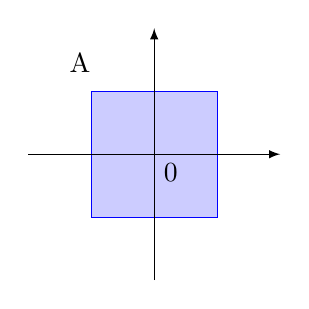
\begin{tikzpicture}[scale=0.8]
        \filldraw[fill=blue!20,draw=blue] (-1,1) rectangle (1,-1);
        \node[below right] at (0,0) {0};
        \draw[-latex] (0,-2) -- (0,2);
        \draw[-latex] (-2,0) -- (2,0);
        \node[below right] at (-1.5,1.75) {A};
    \end{tikzpicture}
    \begin{tikzpicture}[scale=0.8]
        \draw[-latex] (0,-2) -- (0,2);
        \draw[-latex] (-2,0) -- (2,0);
        \node[below right] at (0,0) {0};
        \draw[blue,thick] (-1.5,-2) -- (1,2) node[below,right]{B};
    \end{tikzpicture}
    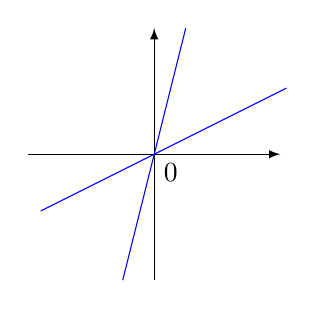
\begin{tikzpicture}[scale=0.8]
            \draw[-latex] (0,-2) -- (0,2);
            \draw[-latex] (-2,0) -- (2,0);
            \node[below right] at (0,0) {0};
            \draw[color=blue,domain=-1.8:2.1] plot(\x,{0.5*(\x)});
            \draw[color=blue,domain=-0.5:0.5] plot(\x,{4*(\x)});
    \end{tikzpicture}
    \begin{tikzpicture}[scale=0.8]
            \draw[-latex] (0,-2) -- (0,2);
            \draw[-latex] (-2,0) -- (2,0);
            \node[below right] at (0,0) {0};
            \filldraw[fill=blue] (0,0) circle [radius=0.1];
            \node[above left] at (0,0) {D};
    \end{tikzpicture}
    \caption{
    不是所有$\R^2$的子集都是子空间。在A,C中, 违反了闭包;
    B不包含$\bs{0}$, 只有D是子空间。
    }
\end{figure}

\begin{remark}
    任意子空间$U \subseteq (\R^n,+,\cdot)$
    是齐次线性方程组$\A\x = \bs{0}, \x \in \R^n$
    的解空间(solutioin space). \hfill $\lozenge$.
\end{remark}

\section{线性无关}

下面,我们将仔细看看我们可以用向量(向量空间的元素)做什么。
特别的,我们可以将向量相加,然后将它们与标量相乘。
闭包性质保证我们最终在同一向量空间中得到另一个向量。
可以找到一组向量,我们可以通过将它们加在一起并缩放它们来表示向量空间中的每个向量。
这组向量是一个基(basis),我们将在 2.6.1 节讨论它们。
在我们到达那里之前,我们需要介绍线性组合(linear combinations)和线性无关(linear independence)的概念。

\begin{definition}[线性组合].
    考虑向量空间$V$和有限数量的向量
    $\x_1,...,\x_k \in V$.
    那么任意以下形式的$\bs{v} \in V$:
    \begin{equation}
        \bs{v} = \lambda_1\x_1 + \cdots
        + \lambda_k \x_k=
        \sum_{i=1}^{k}\lambda_i \x_i \in V
    \end{equation}
    是关于向量$\x_1,...,\x_k$的线性组合,
    其中$\lambda_1,...,\lambda_k \in \R$\marginpar{线性组合}
\end{definition}

$\bs{0}$-向量总是可以被表示为
k个向量$\x_1,...,\x_k$
的线性组合, 因为
$\bs{0} = \sum_{i=1}^{k}0\x_i$总是成立的。
接下来,我们感兴趣的是一组向量的非平凡线性组合来表示$\bs{0}$,
即向量$\x_1,...,\x_k$的线性组合。
,其中并非 (2.65) 中的所有系数$\lambda_i$都是 0。

\begin{definition}[线性无关(相关)].
    让我们考虑一个向量空间$V$,
    其中$k \in \mb{N}$和
    $\x_1,...,\x_k \in V$。
    如果存在非平凡的线性组合,使得
    $\bs{0} = \sum_{i=1}^{k}0\x_i$
    有至少有一个$\lambda_i \neq 0$,
    则向量 $\x_1,...,\x_k \in V$
    是线性相关的。
    如果仅存在平凡解,即$\lambda_1 = ... = \lambda_k = 0$
    那么,
    向量 $\x_1,...,\x_k \in V$
    是线性无关的。
\end{definition}

线性无关是线性代数中最重要的概念之一。
直观地说,一组线性无关向量由没有冗余的向量组成,即,
如果我们从集合中删除这些向量中的任何一个,我们就会失去一些东西。
在接下来的部分中,我们将更多地感受这种直觉。

\begin{example}[线性相关向量].
   地理示例可能有助于阐明线性独立的概念。
   内罗毕(肯尼亚)的一个人在描述基加利(卢旺达)的位置时可能会说,
   “你可以先向西北行驶 506 公里到坎帕拉(乌干达),然后向西南行驶 374 公里,才能到达基加利。”。
   这些信息对于描述基加利的位置足够了,因为地理坐标系可以被认为是一个二维向量空间
   (忽略高度和地球的曲面)。
   此人可能会补充说,“在此以西约 751 公里处。”
   尽管这最后一句是正确的,鉴于先前的信息,这没有必要。,
   (有关说明,请参见图 2.7)。
   在这个例子中,“西北 506 公里”向量(蓝色)和“西南 374 公里”向量(紫色)线性无关。
   这意味着不能用西北向量来描述西南向量,反之亦然。
   然而,第三个“751 km West”向量(黑色)是其他两个向量的线性组合,它使向量集线性相关。
   等效地,给定“西 751 公里”和“西南 374 公里”可以线性组合得到“西北 506 公里”。
\begin{figure}
    \begin{tikzpicture}
        % 引入图片
        \node[anchor=south west,inner sep=0] (image) at (0,0) {
\includegraphics[width=0.9\textwidth]{chapter02/kigali.png}};
        \begin{scope}[x={(image.south east)},y={(image.north west)}]
            % 建立相对坐标系
            % \draw[help lines,xstep=.1,ystep=.1] (0,0) grid (1,1);
            % \foreach \x in {0,1,...,9} { \node [anchor=north] at (\x/10,0) {0.\x}; }
            % \foreach \y in {0,1,...,9} { \node [anchor=east] at (0,\y/10) {0.\y}; }
            % 作图命令
            \node[above] (Nairobi) at (0.85,0.6) {Nairobi};
            \node[below] (Kigali) at (0.05,0.5) {Kigali};
            \node[above] (Kampala) at (0.25,0.8) {Kampala};
            \draw[blue,-latex,thick] (Nairobi) -- node[above]{506 km Northwest}(Kampala);
            \draw[purple,-latex,thick] (Kampala) -- node[above]{374 km Sorthwest}(Kigali);
            \draw[-latex,thick] (Nairobi) -- node[above]{751 km West}(Kigali);
            \draw[purple,-latex,thick] (Nairobi) -- node[above]{374 km Sorthwest} (0.65, 0.3);
        \end{scope}
    \end{tikzpicture}
    \caption{二维空间中线性相关向量的地理例子(基本方向粗略近似)}
\end{figure}
\end{example}

\begin{remark}
    以下性质在确定向量是否是线性无关是非常有用:
    \begin{itemize}
        \item $k$个向量不是线性相关就是线性无关, 没有第三种选择。
        \item 如果向量$\x_1,...,\x_k$中至少
              有一个向量是$\bs{0}$, 那他们就是线性相关。
              如果有两个向量相同也是这样的。
        \item 向量$\{\x_1,...,\x_k : \x_i \neq \bs{0}, i = 1, ...,k\}, k \geqslant 2$,
              线性相关, 当且仅当(至少)其中一个向量是其他向量的线性组合。
              特别地,如果一个向量是另一个向量的倍数,
              即$\x_i = \lambda \x_j$,
              $\lambda \in \R$
              那么集合$\{x_1,..., x_k : x_i \neq \bs{0}, i = 1, ..., k\}$
              是线性相关的。
        \item 一种检查向量$\x_1,...,\x_k \in V$是否线性无关的特殊方法是使用高斯消元法:
              将所有向量写成矩阵 $\A$ 的列并进行高斯消元,直到矩阵为行阶梯形(这里不需要简约行阶梯形):
              \begin{itemize}
                  \item 主元列表示向量,它们与左侧的向量线性无关。
                        请注意,在构建矩阵时存在向量的排序。
                  \item 非主元列可以表示为其左侧主元列的线性组合。
                        例如,这个行阶梯形
                        \begin{equation}
                            \begin{bmatrix}
                                1 & 3 & 0 \\
                                0 & 0 & 2
                            \end{bmatrix}
                        \end{equation}
                        告诉我们第1,3列是主元列。
                        第2列是非主元列因为它是第1列的3倍。
              \end{itemize}
    \end{itemize}
    当且仅当所有列都是主元列时,所有列向量都是线性无关的。
    如果至少有一个非主元列,则这些列(以及相应的向量)是线性相关的。
    \hfill $\lozenge$
\end{remark}

\begin{example}
考虑$\R^4$与
\begin{equation}
    \x_1 =
    \begin{bmatrix}
        1 \\ 2 \\ -3 \\ 4
    \end{bmatrix},
    \x_2 =
    \begin{bmatrix}
        1 \\ 1 \\ 0 \\ 2
    \end{bmatrix},
    \x_3 =
    \begin{bmatrix}
        -1 \\ -2 \\ 1 \\ 1
    \end{bmatrix}.
\end{equation}
为了检查他们是否线性无关, 我们遵循一般方法并解
\begin{equation}
    \lambda_1\x_1 + \lambda_2\x_2 + \lambda_3\x_3 = \lambda_1
    \begin{bmatrix}
        1 \\ 2 \\ -3 \\ 4
    \end{bmatrix} +
    \lambda_2
    \begin{bmatrix}
        1 \\ 1 \\ 0 \\ 2
    \end{bmatrix} +
    \lambda_3
    \begin{bmatrix}
        -1 \\ -2 \\ 1 \\ 1
    \end{bmatrix}
    =\bs{0}
\end{equation}
我们用向量$\x_i,i = 1,2,3$作为一个矩阵的列并应用基本行操作, 直到我们确定主元列:
\begin{equation}
    \begin{bmatrix}
         1 &  1 & -1 \\
         2 &  1 & -2 \\
        -3 &  0 &  1 \\
         4 &  2 &  1 \\
    \end{bmatrix}
    \quad \rightsquigarrow \cdots \rightsquigarrow \quad
    \begin{bmatrix}
         1 &  1 & -1 \\
         0 &  1 &  0 \\
         0 &  0 &  1 \\
         0 &  0 &  0 \\
    \end{bmatrix}.
\end{equation}
这里,矩阵的每一列都是一个主元列。
因此,不存在非平凡解,我们用
$\lambda_1 = 0,\lambda_2 = 0,\lambda_3 = 0$ 来求解方程组。
因此,向量$\x_1,\x_2,\x_3$是线性无关的。
\end{example}

\begin{remark}
    考虑向量空间$V$
    考虑具有$k$个线性无关向量
    $\b_1,...,\b_k$
    的向量空间$V$。
    和$m$个线性组合
    \begin{equation}
    \begin{aligned}
        \x_1 &= \sum_{i=1}^{k}\lambda_{i1}\b_i, \\
                         &\vdots \\
        \x_m &= \sum_{i=1}^{k}\lambda_{im}\b_i, \\
    \end{aligned}
    \end{equation}
    定义$\B = [\b_1,...,\b_k]$
    为矩阵, 其中每一列都是线性独立的向量$\b_1,...,\b_k$, 我们用
    \begin{equation}
        \x_j = \bs{B\lambda}_j,
        \quad
        \bs{\lambda}_j =
        \begin{bmatrix}
            \lambda_{1j} \\
            \vdots \\
            \lambda_{kj} \\
        \end{bmatrix},
        \quad
        j = 1,..., m,
    \end{equation}
    来更简洁的表示他们。

    我们想要测试
    $\x_1,..., \x_m$
    是否线性独立。
    为此,我们遵循当
    $\sum_{j=1}^{m}\psi_j\x_j = \bs{0}$
    时的一般检验方法。
    根据 (2.71),我们得到
    \begin{equation}
       \sum_{j=1}^{m}\psi_j\x_j
       =
       \sum_{j=1}^{m}\psi_j\B\bs{\lambda}_j
       =
       \B\sum_{j=1}^{m}\psi_j\bs{\lambda_j}
    \end{equation}
    这意味着
    $\{\x_1,..., \x_m\}$
    线性无关当且仅当列向量
    $\{\bs{\lambda}_1,..., \bs{\lambda}_m\}$是线性无关的。
    \hfill $\lozenge$
\end{remark}

\begin{remark}
    在向量空间$V$中,
    k个向量$\x_1,...,\x_k$的$m$个线性组合
    是线性相关的, 如果$m > k$. \hfill $\lozenge$
\end{remark}

\begin{example}
考虑一组线性无关向量
$\b_1,\b_2,\b_3,\b_4 \in \R^n$
并且
\begin{equation}
    \begin{aligned}
        \begin{array}{lllllllll}
            \x_1 &=&  \b_1   &-& 2\b_2  &+&\b_3    &-& \b_4 \\
            \x_2 &=&  -4\b_1 &-& 2\b_2  & &                    &+& 4\b_4 \\
            \x_3 &=&  2\b_1  &+& 3\b_2  &-&\b_3    &-& 3\b_4 \\
            \x_4 &=&  17\b_1 &-& 10\b_2 &+&11\b_3  &+& \b_4 \\
        \end{array}
    \end{aligned}
\end{equation}
向量$\x_1,...,\x_4 \in \R^n$线性独立吗?
为了回答这个问题, 我们调查列向量
\begin{equation}
    \left\{
    \begin{bmatrix}
        1 \\ -2 \\ 1 \\ -1
    \end{bmatrix},
    \begin{bmatrix}
        -4 \\ -2 \\ 0 \\ 4
    \end{bmatrix},
    \begin{bmatrix}
        2 \\ 3 \\ -1 \\ -3
    \end{bmatrix},
    \begin{bmatrix}
        17 \\ -10 \\ 11\\ 1
    \end{bmatrix}
    \right\}
\end{equation}
是否是线性独立的。
对应线性方程组的系数矩阵
\begin{equation}
    \A=
    \begin{bmatrix}
        1 & -4 & 2 & 17 \\
        -2 & -2 & 3 & 10 \\
        1 & 0 & -1 & 11 \\
        -1 & 4 & -3 & 1 \\
    \end{bmatrix}
\end{equation}
其简约行阶梯形矩阵
\begin{equation}
    \begin{bmatrix}
        1 & 0 & 0 & -7 \\
        0 & 1 & 0 & -15 \\
        0 & 0 & 1 & -18 \\
        0 & 0 & 0 & 0 \\
    \end{bmatrix}
\end{equation}
我们看到相应的线性方程组是非平凡可解的:
最后一列不是主元列,并且
$\x_4 = −7\x_1 −15\x_2 −18\x_3$。
因此,$\x_1,..., \x_4$是线性相关的,
因为$\x_4$可以表示为$\x_1,...,\x_3$的线性组合。
\end{example}

\section{基与秩}

在向量空间$V$中,我们对向量集合$\mc{A}$特别感兴趣,这些向量集合具有性质:
任何向量$\bs{v} \in V$可以通过$\mc{A}$中向量的线性组合获得。
这些向量是特殊的向量,接下来,我们将表征它们。

\subsection{生成集合与基}

\begin{definition}[生成集合与张成]
    考虑向量空间$V=(\mc{V,+,\cdot})$
    和一组向量$\mc{A}=\{\x_1,...,\x_k\} \subseteq \mc{V}$.
    如果任意向量$\bs{v}\in \mc{V}$能够表示为
    $\x_1,...,\x_k$的线性组合,
    $\mc{A}$称作$V$的一个生成集合(generating set).
    $\mc{A}$向量的所有线性组合的集合称为$\mc{A}$的张成(span).
    如果$\mc{A}$张成向量空间$V$, 我们写作
    $V = \mathrm{span}[\mc{A}]$ 或者
    $V = \mathrm{span}[\x_1,...,\x_k]$.
\end{definition}

生成集合是张成向量(子)空间的向量集,
即每个向量都可以表示为生成集中向量的线性组合。
现在,我们将更具体地描述张成向量(子)空间的最小生成集。

\begin{definition}[基].
    考虑向量空间$V=(\mc{V,+,\cdot})$
    和$\mc{A} \subseteq \mc{V}$.
    $V$的生成集合$\mc{A}$称为最小的(minimal)
    如果不存在更小的集合
    $\tilde{\mc{A}}\subsetneq\mc{A}\subseteq\mc{V}$
    张成$V$.
    任意线性无关的生成集合都是最小的, 称作$V$的基(basis).
\end{definition}

令$V = (\mc{V},+,\cdot)$为向量空间并且
$\mc{B} \subseteq \mc{V}, \mc{B} \neq \emptyset$.
那么, 下面的陈述是等价的:
\begin{itemize}
    \item $\mc{B}$是$V$的一个基。
    \item $\mc{B}$是一个最小生成集合。
    \item $\mc{B}$是$V$中的最大线性无关向量集,添加集合外的任何其他向量将使其线性相关。
    \item 任意向量$\x \in V$是
          $\mc{B}$中向量的线性组合,并且每个线性组合都是唯一的,i.e.
    \begin{equation}
        \x =
        \sum_{i=1}^{k}\lambda_i\b_i =
        \sum_{i=1}^{k}\psi_i\b_i
    \end{equation}
    其中,$\lambda_i, \psi_i \in \R,\b_i \in \mc{B}$
    它遵循$\lambda_i = \psi_i, i = 1,\dots,k$.
\end{itemize}

\begin{example}
    .
    \begin{itemize}
        \item $\R^3$中, 规范/标准基是
        \begin{equation}
            \mc{B} = \left\{
                \begin{bmatrix} 1 \\ 0 \\ 0 \end{bmatrix},
                \begin{bmatrix} 0 \\ 1 \\ 0 \end{bmatrix},
                \begin{bmatrix} 0 \\ 0 \\ 1 \end{bmatrix}
            \right\}
        \end{equation}
        \item $\R^3$中不同的基
        \begin{equation}
           \mc{B}_1 = \left\{
                \begin{bmatrix} 1 \\ 0 \\ 0 \end{bmatrix},
                \begin{bmatrix} 1 \\ 1 \\ 0 \end{bmatrix},
                \begin{bmatrix} 1 \\ 1 \\ 1 \end{bmatrix}
            \right\},
            \mc{B}_2 = \left\{
                \begin{bmatrix} 0.5 \\ 0.8 \\ 0.4 \end{bmatrix},
                \begin{bmatrix} 1.8 \\ 0.3 \\ 0.3 \end{bmatrix},
                \begin{bmatrix} -2.2 \\ -1.3 \\ 3.5 \end{bmatrix}
            \right\}.
        \end{equation}
        \item 集合
        \begin{equation}
           \mc{A} = \left\{
               \begin{bmatrix}
                   1 \\ 2 \\ 3 \\ 4
               \end{bmatrix},
               \begin{bmatrix}
                   2 \\ -1 \\ 0 \\ 2
               \end{bmatrix},
               \begin{bmatrix}
                   1 \\ 1 \\ 0 \\ -4
               \end{bmatrix}
           \right\}
        \end{equation}
        是线性独立的, 但是不是一个生成集合(也不是基):
        例如,向量$[1, 0, 0, 0]^\top$不能通过$\mc{A}$中元素的线性组合获得。
    \end{itemize}
\end{example}

\begin{remark}
    每个向量空间$V$都有一个基$\mc{B}$。
    前面的例子表明向量空间$V$可以有很多基,即没有唯一的基。
    但是,所有基都具有相同数量的元素,即基向量(basis vectors)
    \hfill $\lozenge$
\end{remark}

我们只考虑有限维向量空间$V$。
在这种情况下,$V$的维数是$V$的基向量的数量,我们写成$\dim(V)$。
如果$U \subseteq V$是$V$的子空间,则$\dim(U) \leqslant \dim(V)$
并且当且仅当$U=V$时, $\dim(U) = \dim(V)$.
直觉上,向量空间的维数可以被认为是这个向量空间中独立方向的数量。

\begin{remark}
    向量空间的维数不必是向量中的元素数。
    举个例子, 向量空间
    $V = \spn [\begin{bmatrix} 0 \\ 1 \end{bmatrix}]$
    是一维的, 尽管向量拥有两个元素。\hfill $\lozenge$
\end{remark}

\begin{remark}
   子空间$U$的基$\spn[\bs{x}_1,...,\bs{x}_m] \subseteq \mb{R}^n$
   可以通过执行以下步骤找到:
   \begin{enumerate}
       \item 将张成向量(spanning vectors)写成矩阵$\bs{A}$的列
       \item 确定$\bs{A}$的REF
       \item 与主元列关联的张成向量是$U$的基。
   \end{enumerate}
   \hfill $\lozenge$
\end{remark}

\begin{example}[确定基]
    对于向量子空间$U \subseteq \mb{R}^5$, 被以下向量张成
    \begin{equation}
        \bs{x}_1=
        \begin{bmatrix}
            1 \\ 2 \\ -1 \\ -1 \\ -1
        \end{bmatrix},
        \bs{x}_2=
        \begin{bmatrix}
            2 \\ -1 \\ 1 \\ 2 \\ -2
        \end{bmatrix},
        \bs{x}_3=
        \begin{bmatrix}
            3 \\ -4 \\ 3 \\ 5 \\ -3
        \end{bmatrix},
        \bs{x}_4=
        \begin{bmatrix}
            -1 \\ 8 \\ -5 \\ -6 \\ 1
        \end{bmatrix}
        \in \mb{R}^5,
    \end{equation}
    我们想要找出哪些向量$\bs{x}_1 ,..., \bs{x}_4$是$U$的基。
    为此,我们需要检查$\bs{x}_1 ,..., \bs{x}_4$是否线性无关。
    因此,我们需要解
    \begin{equation}
        \sum_{i=1}^{4} \lambda_i \bs{x}_i = \bs{0},
    \end{equation}
    于是有齐次方程组,其矩阵
    \begin{equation}
        \begin{bmatrix}
            \bs{x}_1 & \bs{x}_2 & \bs{x}_3 & \bs{x}_4
        \end{bmatrix} =
        \begin{bmatrix}
           1 & 2 & 3 & -1 \\
           2 & -1 & -4 & 8 \\
          -1 & 1 & 3 & -5 \\
          -1 & 2 & 5 & -6 \\
          -1 & -2 & -3 & 1 \\
        \end{bmatrix}
    \end{equation}
    根据线性方程组的基本变换规则,我们得到行阶梯形矩阵
    \[
        \begin{bmatrix}
           1 & 2 & 3 & -1 \\
           2 & -1 & -4 & 8 \\
          -1 & 1 & 3 & -5 \\
          -1 & 2 & 5 & -6 \\
          -1 & -2 & -3 & 1 \\
        \end{bmatrix}
        \quad \rightsquigarrow \cdots \rightsquigarrow \quad
        \begin{bmatrix}
           1 & 2 & 3 & -1 \\
           0 & 1 & 2 & -2 \\
           0 & 0 & 0 & 1 \\
           0 & 0 & 0 & 0 \\
           0 & 0 & 0 & 0 \\
        \end{bmatrix}
    \]
    由于主元列表示哪组向量线性无关,
    我们从行阶梯梯形矩阵中看出$\bs{x}_1 , \bs{x}_2 , \bs{x}_4$
    是线性无关的
    (因为线性方程组
    $\lambda_1\bs{x}_1 + \lambda_2\bs{x}_2 + \lambda_4\bs{x}_4 = \bs{0}$
    只能求解为$\lambda_1 = \lambda_2 = \lambda_4 = 0)$。
    因此, $\{\bs{x}_1, \bs{x}_2, \bs{x}_4\}$ 是$U$的基。
\end{example}

\subsection{秩}

矩阵$\bs{A}\in \mb{R}^{m×n}$的线性无关列数等于线性无关行数,
称为$\bs{A}$的秩,记为$\rk(\bs{A})$.\marginpar{秩}

\begin{remark}
    矩阵的秩有一些重要的性质:
    \begin{itemize}
    \item $\rk(\bs{A}) = \rk(\bs{A}^\top)$,即列秩等于行秩。
    \item $\bs{A} \in \mb{R}^{m\times n}$的列
           张成一个子空间$U \subseteq \R^{m\times n}$
           且$\dim(U) = \rk(\bs{A})$.
           稍后我们将把这个子空间称为像(image)或范围(range)。
           可以通过对$\bs{A}$应用高斯消元法来确定主元列,从而找到$U$的基。
    \item $\bs{A} \in \mb{R}^{m\times n}$的行张成子空间
          $W \subseteq \R^n$, 且$\dim(W) = \rk(\bs{A})$.
          $W$的基可以通过对$\bs{A}^\top$应用高斯消元法来找到。
    \item 对于所有$\bs{A} \in \R^{n \times n}$,$\bs{A}$是正规的(可逆的)当且仅当$\rk(\bs{A}) = n$。
    \item 对于所有$\bs{A} \in \mb{R}^{m\times n}$
          和所有 $\bs{b} \in \mb{R}^{m\times n}$
          当且仅当$\rk(\bs{A}) = \rk(\bs{A}|b)$时,
          线性方程组$\A\x = \bs{b}$有解,其中$\bs{A}|\bs{b}$表示增广矩阵。。
    \item 对于$\bs{A} \in \mb{R}^{m\times n}$,
          $\A\x = \bs{0}$的解的子空间维度为
          $n − \rk(\bs{A})$。
          稍后,我们将称这个子空间为核(kernel)或零(null)空间。
    \item 如果矩阵$\bs{A} \in \R^{m\times n}$的秩等于相同维度矩阵的最大可能秩,则该矩阵具有满秩。
          这意味着满秩矩阵的秩是行数和列数中的较小者,即$\rk(A) = \min(m,n)$。
          如果矩阵没有满秩,则称该矩阵是秩亏的(rank deficient)。
    \end{itemize}
    \hfill $\lozenge$
\end{remark}

\begin{example}[秩].\\
    \begin{itemize}
        \item $\A =
        \begin{bmatrix}
            1 & 0 & 1 \\
            0 & 1 & 1 \\
            0 & 0 & 0
        \end{bmatrix}$.
        $\A$有两个线性无关行/列, 所以$\rk(\A) = 2$.
        \item $\A =
        \begin{bmatrix}
            1 & 2 & 1 \\
            -2 & -3 & 1 \\
            3 & 5 & 0
        \end{bmatrix}$
        我们使用高斯消元法来确定秩:
        \begin{equation}
            \begin{bmatrix}
                1 & 2 & 1 \\
                -2 & -3 & 1 \\
                3 & 5 & 0
            \end{bmatrix}
            \quad \rightsquigarrow\cdots\rightsquigarrow\quad
            \begin{bmatrix}
                1 & 2 & 1 \\
                0 & 1 & 3 \\
                0 & 0 & 0
            \end{bmatrix}.
        \end{equation}
        这里, 我们看到线性无关的行列都是$2$, 所以$\rk(\A) = 2$.
    \end{itemize}
\end{example}

\section{线性映射}

接下来,我们将研究保留其结构的向量空间上的映射(mappings),这将使我们能够定义坐标(coordinate)的概念。
在本章的开头,我们说过向量是可以相加并乘以标量的对象,结果对象仍然是向量。
我们希望在应用映射时保留这个属性:考虑两个实向量空间(real vector spaces)$V, W$。
映射$\Phi : V \rightarrow W$保留向量空间的结构,如果
\begin{align}
    \Phi(\x + \y) &= \Phi(\x) + \Phi(y) \\
    \Phi(\lambda\x) &= \lambda\Phi(\x)
\end{align}
对于所有$\x,\y \in V$和$\lambda \in \R$.
我们将其总结为如下定义:
\begin{definition}[线性映射].
   对于向量空间$V,W$, 线性映射$\Phi:V\rightarrow W$称为线性映射
   (或向量空间同态(vector space homomorphism)/线性变换(linear transformation))如果
   \begin{equation}
       \forall \x,\y \in V \forall \lambda,\psi \in \R:
       \Phi(\lambda\x + \psi \y) = \lambda \Phi(\x) + \psi \Phi(\y)
   \end{equation}
\end{definition}

事实证明,我们可以将线性映射表示为矩阵(第 2.7.1 节)。
回想一下,我们还可以收集一组向量作为矩阵的列。
在处理矩阵时,我们必须记住矩阵代表什么:线性映射或向量集合。
我们将在第 4 章中看到更多关于线性映射的内容。
在继续之前,我们将简要介绍特殊映射。

\begin{definition}[单射、满射、双射].
    考虑映射$\Phi:V \rightarrow W$,其中$V, W$可以是任意集合。
    那么$\Phi$被称为
    \begin{itemize}
        \item 单射:如果$\forall \x,\y \in \mc{V}:
               \Phi(\x) = \Phi(\y) \Longrightarrow \x = \y$.
        \item 满射:如果$\Phi(\mc{V})=\mc{W}$.
        \item 双射:如果它既是单射, 也是满射。
    \end{itemize}
\end{definition}

如果$\Phi$是满射,那么$\mc{W}$中的每个元素都可以使用$\Phi$从$\mc{V}$"获得"。
双射$\Phi$可以“撤销(undone)”,即存在映射$\Psi:\mc{W} \rightarrow \mc{V}$
使得$\Psi \circ \Phi(\x) = \x$.
这个映射$\Psi$被称为$\Phi$的逆,通常用$\Phi^{−1}$表示。

通过这些定义,我们介绍向量空间$V$和$W$间线性映射的特殊情况:
\begin{itemize}
    \item 同构(Isomorphism)\marginpar{Isomorphism}   :$\Phi:V \rightarrow W$线性和双射
    \item 内同态(Endomorphism)\marginpar{Endomorphism}:$\Phi:V \rightarrow V$线性
    \item 自同构(Automorphism)\marginpar{Automorphism}:$\Phi:V \rightarrow V$线性和双射
    \item 我们将 $\mathrm{id}_V:V \rightarrow V ,\x \mapsto \x$
          定义为$V$中的恒等映射(identity mapping)或恒等自同构(identity automorphism)。
\end{itemize}

\begin{example}[同态]
    映射$\Phi:\R^2 \rightarrow \mb{C}, \Phi(\x) = x_1 + ix_2$是同态(homomorphism):
    \begin{equation}
        \begin{aligned}
            \Phi\left(
                \begin{bmatrix} x_1 \\ x_2 \end{bmatrix} +
                \begin{bmatrix} y_1 \\ y_2 \end{bmatrix}
                \right) &=
            (x_1 + y_1) + i(x_2 + y_2) = x_1 + ix_2 + y_1 + iy_2 \\
            &= \Phi \left(\begin{bmatrix} x_1 \\ x_2 \end{bmatrix}\right)
            + \Phi \left(\begin{bmatrix} y_1 \\ y_2 \end{bmatrix}\right) \\
            \Phi\left(\lambda \begin{bmatrix} x_1 \\ x_2 \end{bmatrix}\right)
            &= \lambda x_1 + \lambda i x_2 = \lambda(x_1+ix_2)
            = \lambda \Phi\left(\begin{bmatrix} x_1 \\ x_y \end{bmatrix}\right)
        \end{aligned}
    \end{equation}
    这也证明了为什么可以将复数表示为$\R^2$中的元组:
    存在双射线性映射,可将$\R^2$中元组的元素加法转换为具有对应加法的复数集。
    请注意,我们只显示了线性,而不是双射。
\end{example}

\begin{theorem}[Theorem 3.59 in Axler(2015)]
    有限维向量空间$V$和$W$是同构的当且仅当$\dim(V) = \dim(W)$.
\end{theorem}

定理 2.17 指出在两个相同维度的向量空间之间存在线性双射映射。
直观上,这意味着相同维度的向量空间是一种相同的东西,
因为它们可以相互转换而不会产生任何损失。

定理 2.17 也给出了将$\R^{m×n}$($m\times n$矩阵的向量空间)
和$\R^{mn}$(长度为$mn$的向量的向量空间)视为相同的理由,
因为它们的维数是$mn$,并且存在线性的将一个转换为另一个的双射映射。

\begin{remark}
    考虑向量空间$V,W,X$, 那么:
    \begin{itemize}
        \item 对于线性映射$\Phi:V \rightarrow W$和$\Psi:W \rightarrow X$,
              映射$\Psi \circ \Phi:V \rightarrow X$也是线性的。
        \item 如果$\Phi:V \rightarrow W$是同构,那么$\Phi^{−1}:W \rightarrow V$也是同构。
        \item 如果$\Phi:V \rightarrow W, \Psi:V\rightarrow W$是线性的, 那么
              $\Phi + \Psi$和$\lambda \Phi, \lambda \in \R$也是线性的
              \hfill $\lozenge$
    \end{itemize}
\end{remark}

\subsection{线性映射的矩阵表示}

任何$n$-维向量空间与$\R^n$同构(定理 2.17)。
我们考虑一个基${\b_1 ,..., \b_n}$的$n$-维向量空间$V$。
接下来,基向量的顺序将很重要。
因此,我们令
\begin{equation}
    B = (\b_1,\dots,\b_n)
\end{equation}
并且称该$n$-元组为$V$的一个有序基(ordered basis).

\begin{remark}[符号]。
    我们正处于符号变得有点棘手的地步。
    因此,我们在这里总结一部分。
    $B = (\b_1,\dots, \b_n)$是有序基,
    $\mc{B} = \{\b_1,\dots, \b_n\}$是一个(无序)基,
    $\B = [\b_1,\dots, \b_n ]$是一个矩阵,
    其列是向量$\b_1,\dots,\b_n$.
\end{remark}

\begin{definition}[坐标(coordinates)]
    考虑向量空间$V$和$V$的一个有序基$B = (\b_1,\dots, \b_n)$.
    对于所有$\x \in V$,我们得到一个$\x$相对于$B$的唯一的表示(线性组合)
    \begin{equation}
        \x = \alpha_1\b_1 + \dots + \alpha_n\b_n
    \end{equation}
    那么, $\alpha_1,\dots,\alpha_n$是$\x$相对于B的坐标,并且向量
    \begin{equation}
        \bs{\alpha} =
        \begin{bmatrix}
            \alpha_1 \\ \vdots \\ \alpha_n
        \end{bmatrix}
        \in \R^n
    \end{equation}
    是$\x$相对于有序基$B$的坐标向量/坐标表示
\end{definition}

\begin{figure}
    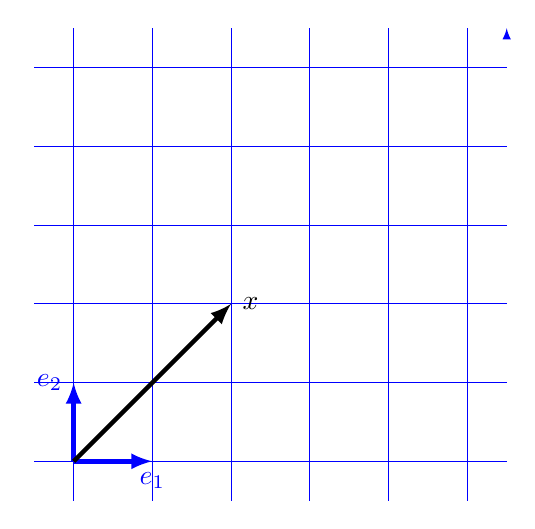
\begin{tikzpicture}[ultra thick, -latex]
        \draw[help lines, blue,thin] (-0.5,-0.5) grid (5.5,5.5);
        \draw[blue] (0,0) -- (1,0) node[below]{$e_1$};
        \draw[blue] (0,0) -- (0,1) node[left]{$e_2$};
        \draw[black] (0,0) -- (2,2) node[right]{$x$};
    \end{tikzpicture}
    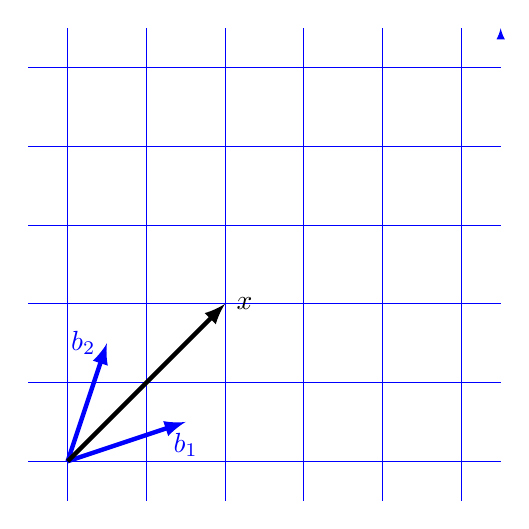
\begin{tikzpicture}[ultra thick, -latex]
        \draw[help lines, blue,thin] (-0.5,-0.5) grid (5.5,5.5);
        \draw[blue] (0,0) -- (1.5,0.5) node[below]{$b_1$};
        \draw[blue] (0,0) -- (0.5,1.5) node[left]{$b_2$};
        \draw[black] (0,0) -- (2,2) node[right]{$x$};
    \end{tikzpicture}
    \caption{由两组基向量定义的两个不同坐标系。
    根据选择的坐标系,向量$\x$具有不同的坐标表示。}
\end{figure}

一个基有效地定义了一个坐标系(coordinate system)。
我们熟悉二维笛卡尔坐标系(Cartesian coordinate system in two dimensions),
它由规范基向量$\e_1,\e_2$张成。
在这个坐标系中,向量$\x \in \R^2$有一个表示,
它告诉我们如何线性组合$\e_1$和$\e_2$以获得$\x$。
然而,$\R^2$的任何基定义了一个有效的坐标系,
并且之前的相同向量$\x$在$(\b_1, \b_2)$基中可能具有不同的坐标表示。
在图 2.8 中,$x$相对于标准基$(\e_1, \e_2)$的坐标是$[2, 2]^\top$。
然而,对于基$(\b_1, \b_2)$,相同的向量$\x$表示为$[1.09, 0.72]^\top$,
即$\x = 1.09\b_1 + 0.72\b_2$。
在下面的部分中,我们将发现如何获得这种表示。

\begin{example}
    让我们看一下几何向量$\x \in \R^2$,
    其相对于$\R^2$的标准基$(\e_1 , \e_2)$的坐标为$[2, 3]^\top$。
    这意味着,我们可以写出$\x = 2\e_1 + 3\e_2$。
    然而,我们不必选择标准基来表示这个向量。
    如果我们使用基向量$\b_1 = [1, -1]^\top, \b_2 = [1, 1]^\top$
    我们将得到坐标$\frac{1}{2}[-1, 5]^\top$来表示相同的向量,
    这是相对于$(\b_1, \b_2)$(见图 2.9)。
\end{example}

\begin{figure}[H]
    \begin{tikzpicture}[-latex,thick]
        \draw[blue] (0,0) -- (1,0) node[below]{$e_1$};
        \draw[blue] (0,0) -- (0,1) node[left]{$e_2$};
        \draw[orange] (0,0) -- (1,-1) node[above right]{$b_1$};
        \draw[orange] (0,0) -- (1,1) node[below right]{$b_2$};
        \draw[black] (0,0) -- (2,3);
        \node [blue] at (-1,3) {$\x = 2\e_1 + 3\e_2$};
        \node [orange] at (-1,2) {$\x = -\frac{1}{2}\b_1 + \frac{5}{2}\b_2$};
    \end{tikzpicture}
    \caption{向量$\x$的不同坐标表示,取决于基的选择。}
\end{figure}

\begin{remark}
    对于 n 维向量空间$V$和$V$的有序基$B$,
    映射$\Phi:\R^n \rightarrow V, \Phi(\e_i) = \b_i, i = 1,\dots, n$是线性的
    (并且由于定理 2.17 是同构的),
    其中$(\e_1,\dots,\e_n)$是$\R^n$的标准基。
    \hfill $\lozenge$
\end{remark}

现在我们准备在矩阵和有限维向量空间之间的线性映射之间建立明确的联系。

\begin{definition}[变换矩阵]
    考虑向量空间$V, W$具有相应的(有序)基
    $B = (\b_1,\dots,\b_n)$和$C = (\c_1,\dots, \c_m )$。
    此外,我们考虑线性映射$\Phi:V \rightarrow W$。
    对于$j \in \{1,\dots, n\}$,
    \begin{equation}
        \Phi(\b_j) = \alpha_{1j}\c_1 + \cdots + \alpha_{mj}\c_m
        = \sum_{i=1}^{m}\alpha_{ij}\c_i
    \end{equation}
    是$\Phi(\b_j)$关于$C$的唯一表示。
    然后,我们称$m \times n$-矩阵$\A_\Phi$,其元素由下式给出
    \begin{equation}
        A_\phi(i,j) = \alpha_{ij},
    \end{equation}
    为$\Phi$的变换矩阵(Transformation Matrix)(相对于$V$的有序基$B$和$W$的有序基$C$)。
\end{definition}

$\Phi(\b_j)$相对于$W$的有序基$C$的坐标是$\A_\Phi$的第$j$列。
考虑(有限维)向量空间$V,W$具有有序基$B,C$和线性映射$\Phi:V \rightarrow W$及其变换矩阵$A_\Phi$。
如果$\hat{\x}̂$ 是 $\x \in V$相对于$B$的坐标向量,
$\hat{\y}$是$\y = \Phi(\x) \in W$相对于$C$的坐标向量,那么
\begin{equation}
    \hat{\y} = \A_\Phi \hat{\x}
\end{equation}
这意味着变换矩阵可用于将关于$V$中有序基的坐标映射到关于$W$中有序基的坐标。

\begin{example}[变换矩阵]
    考虑同态$\Phi:V \rightarrow W$和
    $V$的有序基$B = (\b_1,\dots, \b_3)$和
    $W$的有序基$C = (\c_1,\dots, \c_4)$。
    \begin{equation}
        \begin{aligned}
            \Phi(\b_1) &= \c_1  - \c_2 + 3\c_3 -  \c_4 \\
            \Phi(\b_2) &= 2\c_1 + \c_2 + 7\c_3 + 2\c_4 \\
            \Phi(\b_2) &=       3\c_2 +  \c_3 + 4\c_4 \\
        \end{aligned}
    \end{equation}
    关于B和C的变化矩阵$\A_\Phi$满足
    $\Phi(\b_k) = \sum_{1=1}^{4}\alpha_{ik}\c_i$
    其中$k=1,\dots,3$, 并给出
    \begin{equation}
        \A_\Phi =
        [\bs{\alpha}_1,\bs{\alpha}_2,\bs{\alpha}_3]=
        \begin{bmatrix}
            1 & 2 & 0 \\
            -1 & 1 & 3 \\
            3 & 7 & 1 \\
            -1 & 2 & 4
        \end{bmatrix},
    \end{equation}
    其中$\bs{\alpha}_j,j = 1, 2, 3$是$\Phi(\b_j)$相对于$C$的坐标向量。
\end{example}

\begin{example}[向量的线性变换]
    \begin{figure}[H]
        \subfigure[原始数据]{
            \begin{tikzpicture}
                \draw (-1,0) -- (1,0);
                \draw (0,-1) -- (0,1);
            \end{tikzpicture}
        }
        \subfigure[旋转45度]{
            \begin{tikzpicture}
                \draw (-1,0) -- (1,0);
                \draw (0,-1) -- (0,1);
            \end{tikzpicture}
        }
        \subfigure[伸缩水平轴]{
            \begin{tikzpicture}
                \draw (-1,0) -- (1,0);
                \draw (0,-1) -- (0,1);
            \end{tikzpicture}
        }
        \subfigure[一般线性映射]{
            \begin{tikzpicture}
                \draw (-1,0) -- (1,0);
                \draw (0,-1) -- (0,1);
            \end{tikzpicture}
        }
        \caption{(a) 中用点表示的向量线性变换的三个例子;}
    \end{figure}
    我们考虑$R^2$中一组向量的三个线性变换,其变换矩阵为
    \begin{equation}
        \A_1 =
        \begin{bmatrix}
            \cos(\frac{\pi}{4}) & -\sin(\frac{\pi}{4}) \\
            \sin(\frac{\pi}{4}) & \cos(\frac{\pi}{4})
        \end{bmatrix},
        \A_2 =
        \begin{bmatrix}
            2 & 0 \\
            0 & 1
        \end{bmatrix},
        \A_3 =
        \frac{1}{2}
        \begin{bmatrix}
            3 & -1 \\
            1 & -1
        \end{bmatrix}.
    \end{equation}
    图 2.10 给出了一组向量的线性变换的三个例子。
    图 2.10(a) 显示了$\R^2$中的 400 个向量,每个向量由相应$(x_1 , x_2 )$坐标处的点表示。
    矢量排列在一个正方形中。
    当我们使用(2.97)中的矩阵$\A_1$对这些向量中的每一个进行线性变换时,我们得到图 2.10(b)中的旋转正方形。
    如果我们应用由$\A^2$表示的线性映射, 我们将获得图 2.10(c) 中的矩形, 其中每个$x_1$坐标被拉伸 2倍。
    图 2.10(d) 显示了使用$\A_3$进行线性变换时图 2.10(a) 中的原始正方形, 它是反射、旋转和拉伸的组合。
\end{example}

\subsection{变基/基变换(basis change)}

接下来,我们将仔细研究如果我们改变$V$和$W$中的基,
线性映射$\Phi:V \rightarrow W$的变换矩阵如何改变的。
考虑$V$的两个有序基
\begin{equation}
    B = (\b_1,\dots,\b_n),\quad
    \tilde{B} = (\tilde{\b}_1,\dots,\tilde{\b}_n)
\end{equation}
和$W$的两个有序基
\begin{equation}
    C = (\c_1,\dots,\c_m),\quad
    \tilde{C} = (\tilde{\c}_1,\dots,\tilde{\c}_n)
\end{equation}
此外,$\A_\Phi \in \R^{m \times n}$是
线性映射$\Phi:V \rightarrow W$对基$B$和$C$的变换矩阵,
$\tilde{\A}_\Phi \in \R^{m \times n}$
是对$\tilde{B}$和$\tilde{C}$的对应变换映射。
我们将研究$\A$和$\tilde{}{\A}$是如何相互联系的,
即,如果我们选择执行从$B, C$到$\tilde{B}, \tilde{C}$的基变换,
我们如何/是否可以将$\A_\Phi$转换为$\tilde{\A}_\Phi$。
\begin{remark}
    我们有效地获得了恒等映射$\mathrm{id}_V$的不同坐标表示。
    在图2.9的上下文中,这意味着将关于$(\e_1,\e_2)$的坐标
    映射到关于$(\b_1, \b_2)$的坐标而不改变向量$\x$。
    通过改变基和相应的向量表示,
    关于这个新基的变换矩阵可以有一个特别简单的形式,
    可以允许直接计算。 \hfill $\lozenge$
\end{remark}

\begin{example}[基变换]
    考虑相对于$\R^2$中规范基的变换矩阵
    \begin{equation}
            \A =
        \begin{bmatrix}
            2 & 1 \\ 1 & 2
        \end{bmatrix}
    \end{equation}
    如果我们定义一个新基
    \begin{equation}
        B =(
        \begin{bmatrix} 1 \\ 1 \end{bmatrix},
        \begin{bmatrix} 1 \\ -1 \end{bmatrix}
        )
    \end{equation}
    我们得到一个相对于$B$的对角线变换矩阵
    \begin{equation}
        \tilde{\A}=
        \begin{bmatrix}
            3 & 0 \\ 0 & 1
        \end{bmatrix}
    \end{equation}
    这比$\A$更好用
\end{example}

在下文中,我们将研究将一个基的坐标向量转换为关于不同基的坐标向量的映射。
我们将首先陈述我们的主要结果,然后提供解释。

\begin{theorem}[基变换]
    对于线性映射$\Phi:V\rightarrow W$,$V$的有序基
    \begin{equation}
        B = (\b_1, \dots, \b_n),\quad
        \tilde{B} = (\tilde{\b}_1, \dots, \tilde{\b}_n)
    \end{equation}
    和$W$的有序基
    \begin{equation}
        C = (\c_1, \dots, \c_n),\quad
        \tilde{C} = (\tilde{\c}_1, \dots, \tilde{\c}_n)
    \end{equation}
    以及关于$B$和$C$的变换矩阵$\A_\Phi$,
    关于$\tilde{B}$和$\tilde{C}$的变换矩阵$\tilde{\A}_\Phi$
    \begin{equation}
        \tilde{\A}_\Phi = \bs{T}^{-1}\A_\Phi\bs{S}.
    \end{equation}
    这里,$\bs{S} \in \R^{n \times n}$是$\id_V$的变换矩阵,
    将关于$\tilde{B}$的坐标映射到关于$B$的坐标,
    $\bs{T} \in \R^{m \times m}$是$\id_W$的变换矩阵,
    将关于$\tilde{C}$的坐标映射到$C$的坐标。
\end{theorem}

\begin{proof}
    根据Drumm 和 Weil (2001),
    我们可以将$V$的新基$\tilde{B}$的向量写成$B$的基向量的线性组合,
    使得
    \begin{equation}
        \tilde{\b}_j = s_{1j}\b_1 + \cdots + s_{nj}\b_n =
        \sum_{i=1}^{n} s_{ij}\b_{j},
        \quad j = 1,\dots, n.
    \end{equation}
    类似的,我们将$W$的新基向量$\tilde{C}$写成$C$的基向量的线性组合,得到
    \begin{equation}
        \tilde{\c}_k = t_{1k}\c_1 + \cdots + t_{mk}\c_m =
        \sum_{l=1}^{n} t_{lk}\c_{l},
        \quad k = 1,\dots, m.
    \end{equation}
    我们将$\bs{S}=((s_{ij})) \in \R^{n \times n}$
    定义为将关于$\tilde{B}$的坐标映射到关于$B$的坐标的变换矩阵,
    $\bs{T}= ((t_{lk})) \in \R ^ {m\times m}$作为将关于$\tilde{C}$的坐标映射到到关于$C$的坐标。
    特别地,$\bs{S}$的第$j$列是$\tilde{\b}_j$相对于$B$的坐标表示,
    $\bs{T}$的第k列是$\tilde{\c}_k$相对于$C$的坐标表示。
    请注意,$\bs{S}$和$\bs{T}$都是正规的。

    我们将从两个角度来看$\Phi(\tilde{\b}_j)$。
    首先,应用映射$\Phi$,我们得到所有$j = 1,\dots, n$
    \begin{equation}
        \Phi(\tilde{\b}_j) =
        \sum_{k=1}^{m}
        \underbrace{\tilde{a}_{kj} {\color{blue}\tilde{\c}_k}}_{\in W}
        \overset{(2.107)}{=}
        \sum_{k=1}^{m} \tilde{a}_{kj}
        {\color{blue} \sum_{l=1}^{m}t_{lk}\c_l}
        =
        \sum_{l=1}^{m}
        \left(
            \sum_{k=1}^{m} t_{lk} \tilde{a}_{kj}
        \right)
        \c_l,
    \end{equation}
    这里我们首先将新的基向量$\tilde{\c}_k \in W$
    表示为基向量$\c_l \in W$的线性组合,然后交换求和的顺序。

    或者,当我们将$\tilde{\b}_j \in V$表示为$\b_j \in V$的线性组合时,
    我们得到
    \begin{subequations}
        \begin{equation}
        \Phi({\color{blue}\tilde{\b}_j})
        \overset{(2.106)}{=}
        \Phi
        \left(
            {\color{blue}
            \sum_{i=1}^{n}s_{ij}\b_i
            }
        \right)
        =
        \sum_{i=1}^{n} s_{ij}
        {\color{red}
        \Phi(\b_i)
        }
        =
        \sum_{i=1}^{n} s_{ij}
        \sum_{l=1}^{m}
        {\color{red}
        a_{li} \c_l
        }
        \end{equation}
        \begin{equation}
        =
        \sum_{l=1}^{m} \left(\sum_{i=1}^{n}a_{li} s_{ij}\right)
        \c_l,\quad j = 1,\dots, n,
        \end{equation}
    \end{subequations}
   这里我们利用了$\Phi$的线性(linearity).比较(2.108)和(2.109b),
   它有: 对于所有$j=1,\dots,n$和$l=1,\dots,m$
   \begin{equation}
       \sum_{k=1}^{m}t_{lk} \tilde{a}_{kj} =
       \sum_{i=1}^{n}a_{li} {s}_{ij}
   \end{equation}
   因此:
   \begin{equation}
       \T\tilde{\A}_\Phi = \A_\Phi\bs{S}\in \R^{m \times n},
   \end{equation}
   使得
   \begin{equation}
       \tilde{\A}_\Phi = \T^{-1} \A_\Phi \bs{S},
   \end{equation}
   这就证明了定理2.20. \hfill $\square$
\end{proof}

定理 2.20 告诉我们,
随着$V$($B$替换为 $\tilde{B}$)和$W$($C$ 替换为 $\tilde{C}$)的基变化,
线性映射$\Phi:V \rightarrow W$的变换矩阵$\A_\Phi$被等效矩阵$\tilde{\A}_\Phi$替换为
\begin{equation}
    \tilde{\A}_\Phi = \T^{-1} \A_\Phi \bs{S},
\end{equation}
图 2.11 说明了这种关系:
考虑同态$\Phi:V \rightarrow W$和
$V$的有序基$B, \tilde{B}$,以及$W$的有序基$C,\tilde{C}$。
映射$\Phi_{CB}$是$\Phi$的实例化,
并将$B$的基向量映射到$C$的基向量的线性组合。
假设我们知道相对于有序基$B,C$的$\Phi_{CB}$的变换矩阵$\A_\Phi$。
当我们在$V$中执行从$B$到$\tilde{B}$以及在$W$中从$C$到$\tilde{C}$的基变换时,
我们可以像下面这样确定相应的变换矩阵$\tilde{\A}_\Phi$:
首先,我们找到线性映射$\Psi_{B \tilde{B}}:V \rightarrow V$的矩阵表示,
它将关于新基$\tilde{B}$的坐标映射到相对于“旧”基$B$(在V中)的(唯一)坐标。
然后,我们使用$\Phi_{CB}:V \rightarrow W$的变换矩阵$\A_\Phi$
将这些坐标映射到$W$中相对于$C$的坐标上。
最后,我们使用线性映射$\Xi_{\tilde{C}C}:W \rightarrow W$
将关于$C$的坐标映射到关于$\tilde{C}$的坐标。
因此,我们可以将线性映射$\Phi_{\tilde{C}\tilde{B}}$
表示为涉及“旧”基的线性映射的组合:
\begin{equation}
    \Phi_{\tilde{C}\tilde{B}}=
    \Xi_{\tilde{C}C} \circ \Phi_{CB} \circ \Psi_{B\tilde{B}}=
    \Xi_{C\tilde{C}}^{-1} \circ \Phi_{CB} \circ \Psi_{B\tilde{B}}
\end{equation}
具体来说,我们使$\Psi_{B\tilde{B}} = \id_V$
和$\Xi_{C\tilde{C}}^{-1} = \id_W$,
即,将向量映射到它们自身上的恒等映射,但关于不同的基。

\begin{figure}
    \begin{tikzpicture}[-latex]
        \node at (-3,3) {向量空间};
        \node at (-3,1) {有序基};
        \node (V)  at (0,3) {$V$};
        \node (W)  at (3,3) {$W$};
        \node[blue] (B)  at (0,2) {$B$};
        \node[blue] (tB) at (0,0) {$\tilde{B}$};
        \node[blue] (C)  at (3,2) {$C$};
        \node[blue] (tC) at (3,0) {$\tilde{C}$};
        \draw (V) --node[above]{$\Phi$} (W);
        \draw[ultra thick] (B) --node[above]{$\Phi_{CB}$} node[below,red]{$\A_\Phi$} (C);
        \draw (tB) --node[left]{$\Psi_{B\tilde{B}}$} node[right,red]{$\bs{S}$} (B);
        \draw (tB) --node[above,red]{$\tilde{\A}_\Phi$} node[below]{$\Phi_{\tilde{C}\tilde{B}}$} (tC);
        \draw (tC) --node[left,red]{$\T$} node[right]{$\Xi_{C\tilde{C}}$} (C);
    \end{tikzpicture}
    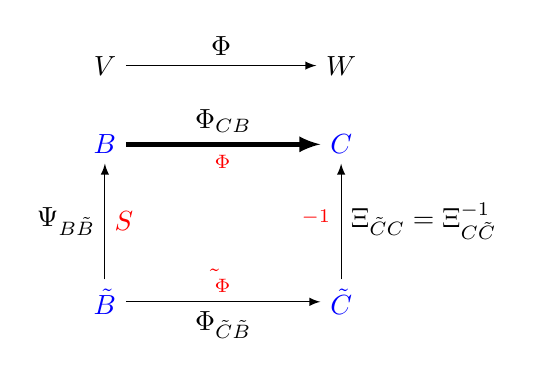
\begin{tikzpicture}[-latex]
        \node (V)  at (0,3) {$V$};
        \node (W)  at (3,3) {$W$};
        \node[blue] (B)  at (0,2) {$B$};
        \node[blue] (tB) at (0,0) {$\tilde{B}$};
        \node[blue] (C)  at (3,2) {$C$};
        \node[blue] (tC) at (3,0) {$\tilde{C}$};
        \draw (V) --node[above]{$\Phi$} (W);
        \draw[ultra thick] (B) --node[above]{$\Phi_{CB}$} node[below,red]{$\A_\Phi$} (C);
        \draw (tB) --node[left]{$\Psi_{B\tilde{B}}$} node[right,red]{$\bs{S}$} (B);
        \draw (tB) --node[above,red]{$\tilde{\A}_\Phi$} node[below]{$\Phi_{\tilde{C}\tilde{B}}$} (tC);
        \draw (tC) --node[left,red]{$\T^{-1}$} node[right]{$\Xi_{\tilde{C}C}=\Xi_{C\tilde{C}}^{-1}$} (C);
    \end{tikzpicture}
    \caption{
        对于同态$\Phi:V \rightarrow W$
        以及$V$的有序基$B, \tilde{B}$,
        $W$的有序基$C,\tilde{C}$(用蓝色标记),
        我们可以将关于基$\tilde{B}, \tilde{C}$的映射$\Phi_{\tilde{C}\tilde{B}}$
        等价地表示为同态
        $\Phi_{\tilde{C}\tilde{B}} = \Xi_{\tilde{C}C} \circ \Phi_{CB} \circ \Psi_{B \tilde{B}}$关于下标中的基。
        相应的变换矩阵为红色。
    }
\end{figure}

\begin{definition}[等价\footnotemark].
    两个矩阵$\A,\tilde{\A} \in \R^{m \times n}$是等价(Equivalence)的, 如果存在正规矩阵
    $\bs{S} \in \R^{n \times n}$并且$\tilde{\A} = \bs{S}^{-1} \A \bs{S}$
    \footnotetext{
        译者注:两个矩阵等价当且仅当:
        \begin{itemize}
            \item 其中一者能够经过若干次初等行或列变换变成另一者。
            \item 它们有相同的秩
        \end{itemize}
    }
    \footnote{该定义其实是相似矩阵的定义.}
\end{definition}
\begin{remark}
    相似矩阵(similar matrices)总是等价的。 然而,等价矩阵不一定相似。
    \hfill $\lozenge$
\end{remark}

\begin{remark}
    考虑向量空间$V, W, X$。
    从定理 2.17 后面的注解,
    我们已经知道对于线性映射$\Phi:V \rightarrow W$和
    $\Psi:W \rightarrow X$,
    映射$\Psi \circ \Phi:V \rightarrow X$也是线性的。
    使用对应映射的变换矩阵$\A_\Phi$和$\A_\Psi$,
    整个变换矩阵为$\A_{\Psi \circ \Phi} = \A_\Psi \A_\Phi$。
    \hfill $\lozenge$
\end{remark}

有鉴于此,我们可以从组合线性映射的角度来看基的变化:
\begin{itemize}
    \item $\A_\Phi$是线性映射$\Phi_{CB}:V \rightarrow W$相对于基$B, C$的变换矩阵。
    \item $\tilde{\A}_\Phi$是线性映射$\Phi_{\tilde{C} \tilde{B}}:V \rightarrow W$相对于基$\tilde{B}, \tilde{C}$的变换矩阵。
    \item $\bs{S}$是线性映射$\Phi_{B\tilde{B}}:V \rightarrow V$(自同构)的变换矩阵,它根据$B$表示$\tilde{B}$。
    通常,$\Psi = \id_V$是$V$中的恒等映射。
    \item $\bs{T}$是线性映射$\Xi_{C\tilde{C}}:W \rightarrow W$(自同构)的变换矩阵,它根据$C$表示$\tilde{C}$。
    通常,$\Xi = \id_W$是$W$中的恒等映射。
\end{itemize}
如果我们(非正式地)只根据基数写下变换,那么
$\A_\Phi : B \rightarrow C,\quad\tilde{\A}_\Phi : \tilde{B} \rightarrow \tilde{C},\quad\bs{S}: \tilde{B} \rightarrow B,\quad\T : \tilde{C} \rightarrow C,\quad\T^{-1}: C \rightarrow \tilde{C} $
\begin{align}
    \tilde{B} \rightarrow \tilde{C} &=
    {\color{blue} \tilde{B} \rightarrow B}
    {\color{red}\rightarrow C}
    \rightarrow \tilde{C}\\
    \tilde{\A}_\Phi &= \T^{-1}
    {\color{red}\A_\Phi}
    {\color{blue}\S}
\end{align}
请注意,(2.116)中的执行顺序是从右到左,
因为向量在右侧相乘,
因此
$\x \mapsto \S\x
\mapsto \A_\Phi (\S\x)
\mapsto \T^{-1}(\A_\Phi (\S\x)) = \tilde{\A}_\Phi \x$

\begin{example}[基变换]
    考虑线性映射$\Phi:\R^3 \rightarrow \R^4$, 其变换矩阵为
    \begin{equation}
        \A_\Phi =
        \begin{bmatrix}
            1 & 2 & 0 \\
           -1 & 1 & 3 \\
            3 & 7 & 1 \\
           -1 & 2 & 4 \\
        \end{bmatrix}
    \end{equation}
    关于标准基
    \begin{equation}
        B = (
            \begin{bmatrix} 1 \\ 0 \\ 0 \end{bmatrix},
            \begin{bmatrix} 0 \\ 1 \\ 0 \end{bmatrix},
            \begin{bmatrix} 0 \\ 0 \\ 1 \end{bmatrix}
        ), \quad
        C = (
            \begin{bmatrix} 1 \\ 0 \\ 0 \\ 0 \end{bmatrix},
            \begin{bmatrix} 0 \\ 1 \\ 0 \\ 0 \end{bmatrix},
            \begin{bmatrix} 0 \\ 0 \\ 1 \\ 0 \end{bmatrix},
            \begin{bmatrix} 0 \\ 0 \\ 0 \\ 1 \end{bmatrix}
        ).
    \end{equation}
    我们寻求关于以下新基的$\Phi$的变换矩阵$\tilde{\A}_\Phi$
    \begin{equation}
        B = (
            \begin{bmatrix} 1 \\ 1 \\ 0 \end{bmatrix},
            \begin{bmatrix} 0 \\ 1 \\ 1 \end{bmatrix},
            \begin{bmatrix} 1 \\ 0 \\ 1 \end{bmatrix}
        ), \in \R^3,
        \quad
        C = (
            \begin{bmatrix} 1 \\ 1 \\ 0 \\ 0 \end{bmatrix},
            \begin{bmatrix} 1 \\ 0 \\ 1 \\ 0 \end{bmatrix},
            \begin{bmatrix} 0 \\ 1 \\ 1 \\ 0 \end{bmatrix},
            \begin{bmatrix} 1 \\ 0 \\ 0 \\ 1 \end{bmatrix}
        ).
    \end{equation}
    然后,
    \begin{equation}
        \S =
        \begin{bmatrix}
            1 & 0 & 1 \\
            1 & 1 & 0 \\
            0 & 1 & 1
        \end{bmatrix}, \quad
        \T =
        \begin{bmatrix}
            1 & 1 & 0 & 1 \\
            1 & 0 & 1 & 0 \\
            0 & 1 & 1 & 0 \\
            0 & 0 & 0 & 1
        \end{bmatrix},
    \end{equation}
    其中$\S$的第$i$列是$\tilde{\b}_i$关于$B$的基向量的坐标表示。
    由于$B$是标准基,所以坐标表示很容易找到。
    对于基$B$,我们需要求解一个线性方程组来找到$\lambda_i$,使得
    $\sum_{i=1}^3 \lambda_i \tilde{\b}_i, j = 1,\dots, 3$.
    类似地,$T$的第$j$列是$\tilde{c}_j$关于$C$的基向量的坐标表示。

    因此, 我们有
    \begin{subequations}
        \begin{align}
        \tilde{\A}_\Phi &= \T^{-1} \A_\Phi \S =
        \frac{1}{2}
        \begin{bmatrix}
            1 &  1 & -1 & -1 \\
            1 & -1 &  1 & -1 \\
           -1 &  1 &  1 &  1 \\
            0 &  0 &  0 &  2
        \end{bmatrix}
        \begin{bmatrix}
            3 & 2 & 1 \\
            0 & 4 & 2 \\
           10 & 8 & 4 \\
            1 & 6 & 3
        \end{bmatrix}
        \\&=
        \begin{bmatrix}
            -4 & -4 & -2 \\
             6 &  0 &  0 \\
             4 &  8 &  4 \\
             1 &  6 &  3 \\
        \end{bmatrix}
        \end{align}
    \end{subequations}
\end{example}

在第 4 章中,我们将能够利用基变换的概念来找到一个基,
关于该基,内同态的变换矩阵具有特别简单的(对角线)形式。
在第 10 章中,我们将研究一个数据压缩问题,并找到一个方便的基,
我们可以将数据投影(project)到该基上,同时最大限度地减少压缩损失。

\subsection{像与核}

线性映射的像(image)和核(kernel)是具有某些重要性质的向量子空间。
下面,我们将更详细地描述它们。

\begin{definition}[像与核]
    对于$\Phi:V \rightarrow W$, 我们定义核/零空间(kernel/null space)
    \begin{equation}
        \ker(\Phi) := \Phi^{-1}(\0_W) =
        \{
            \v \in V : \Phi(\v) = \0_W
        \}
    \end{equation}
    定义像(image/range)
    \begin{equation}
        \Im(\Phi) := \Phi(V) =
        \{
            \w \in W |
            \exists \v \in V :
            \Phi(\v) = \w
        \}
    \end{equation}
    我们也分别称$V$和$W$为$\Phi$的域(domain)和陪域(codomain)。
\end{definition}

直观地, 核是一组向量$\v \in V$,$\Phi$将其映射到单位元$\0_W \in W$上。
像是一组向量$\w \in W$, 可以通过$\Phi$从$V$中的任何向量“到达(reached)”。
图 2.12 给出了解释。

\begin{figure}
    \begin{tikzpicture}
        \filldraw[fill=yellow] (0,0) ellipse [x radius=2,y radius=3];
        \filldraw[fill=orange!40] (0,0) ellipse [x radius=1.5,y radius=2];
        \filldraw[fill=blue!20] (9,0) ellipse [x radius=2.2,y radius=3];
        \filldraw[fill=yellow] (9,0) ellipse [x radius=1.2,y radius=1.7];
        \filldraw (0.5,-0.5) circle [radius=0.05] node[above right]{$\0_V$};
        \filldraw (9.5,-0.5) circle [radius=0.05] node[above right]{$\0_W$};
        \node at (-0.5,1) {$\ker(\Phi)$};
        \node at (9,1) {$\Im(\Phi)$};
        \draw[dashed] (0,2) -- (9.5,-0.5);
        \draw[dashed] (0,-2) -- (9.5,-0.5);
        \draw[dashed] (0,3) -- (9,1.7);
        \draw[dashed] (0,-3) -- (9,-1.7);
        \node at (-1,4) {$V$};
        \node at (10,4) {$W$};
        \node at (5,4) {$\Phi:V \rightarrow W$};
    \end{tikzpicture}
    \caption{线性映射的核和像$\Phi : V \rightarrow W$。}
\end{figure}

\begin{remark}
    考虑线性映射$\Phi : V \rightarrow W$, 其中$V,W$是向量空间。
    \begin{itemize}
        \item 它总是有$\Phi(\0_V) = \0_W$,因此,$\0_V \in \ker(\Phi)$。特别的,零空间永远不会为空。
        \item $\Im(\Phi) \subseteq W$是$W$的子空间, 并且$\ker(\Phi) \subseteq V$是$V$的子空间。
        \item $\Phi$是单射(一对一)当且仅当 $\ker(\Phi) = \{\0\}$。
        \hfill $\lozenge$
    \end{itemize}
\end{remark}

\begin{remark}[零空间和列空间(Column Space)]
    让我们考虑$\A \in \R^{m \times n}$
    和线性映射$\Phi : \R^n \rightarrow \R^m, \x \mapsto \A\x$.
    \begin{itemize}
        \item 对于$\A = [\a_1, \dots, \a_2]$, 其中$\a_i$是$\A$的列, 我们有
        \begin{subequations}
            \begin{align}
                \Im(\Phi) &= \{\A\x: \x \in \R^n\}
                = \left\{
                    \sum_{i=1}^{n} x_i \a_i : x_1, \dots, x_n \in \R
                \right\}\\
                &= \spn[\a_1,\dots,\a_n] \subseteq \R^m,
            \end{align}
        \end{subequations}
        即,像是$A$的列的张成,也称为列空间(column space)。
        因此,列空间(像)是$\R^m$的子空间,其中$m$是矩阵的“高度”。
        \item $\rk(\A) = \dim(\Im(\Phi))$.
        \item 核/零空间$\ker(\Phi)$是线性方程组$\A\x = 0$的齐次线性方程组的一般解,并包含$\R_n$中产生$\0 \in \R^m$的元素的所有可能的线性组合。
        \item 核是$\R^n$的子空间,其中$n$是矩阵的“宽度”。
        \item 核关注列之间的关系,我们可以用它来确定我们是否/如何将一列表示为其他列的线性组合。
        \hfill $\lozenge$
    \end{itemize}
\end{remark}

\begin{example}[线性映射的像与核]
    \begin{subequations}
    \begin{align}
        \Phi:\R^4 \rightarrow \R^2,
        \begin{bmatrix}
            x_1 \\ x_2 \\ x_3 \\ x_4 \\
        \end{bmatrix}
        \mapsto
        \begin{bmatrix}
            1 & 2 & -1 & 0 \\
            1 & 0 & 0 & 1
        \end{bmatrix}
        \begin{bmatrix}
            x_1 \\ x_2 \\ x_3 \\ x_4 \\
        \end{bmatrix}
        =
        \begin{bmatrix}
            x_1 + 2x_2 - x_3 \\
            x_1 + x_4
        \end{bmatrix}\\
        =
        x_1 \begin{bmatrix} 1 \\ 1 \end{bmatrix}
        x_2 \begin{bmatrix} 2 \\ 0 \end{bmatrix}
        x_3 \begin{bmatrix} -1 \\ 0 \end{bmatrix}
        x_4 \begin{bmatrix} 0 \\ 1 \end{bmatrix}
    \end{align}
    \end{subequations}
    是线性的。为了确定$\Im(\Phi)$,我们可以取变换矩阵的列的张成并得到
    \begin{equation}
        \Im(\Phi) = \spn[
            \begin{bmatrix} 1 \\ 1 \end{bmatrix},
            \begin{bmatrix} 2 \\ 0 \end{bmatrix},
            \begin{bmatrix}-1 \\ 0 \end{bmatrix},
            \begin{bmatrix} 0 \\ 1 \end{bmatrix}
        ]
    \end{equation}
    为了计算$\Phi$的核(零空间),
    我们需要求解$\A\x = \0$,即我们需要求解齐次方程组。
    为此,我们使用高斯消元法将$\A$转换为简约行阶梯形:
    \begin{equation}
        \begin{bmatrix}
            1 & 2 & -1 & 0 \\
            1 & 0 & 0 & 1
        \end{bmatrix}
        \quad \rightsquigarrow \cdots \rightsquigarrow \quad
        \begin{bmatrix}
            1 & 0 & 0 & 1 \\
            0 & 1 & -\frac{1}{2} & -\frac{1}{2}
        \end{bmatrix}.
    \end{equation}
    该矩阵采用简约行阶梯形,我们可以使用负一技巧来计算内核的基(参见第 2.3.3 节)。
    或者,我们可以将非主元列(第 3 列和第 4 列)表示为主元列(第 1 列和第 2 列)的线性组合。
    第三列$\a_3$相当于$-\frac{1}{2}$乘以第二列$\a_2$。
    因此,$\0 = \a_3 + \frac{1}{2} \a_2$。
    以同样的方式,我们看到$\a_4 = \a_1 − \frac{1}{2} \a_2$,
    因此,$\0 = \a_1 − \frac{1}{2} \a_2 − \a_4$。
    总的来说,这给了我们内核(零空间)为
    \begin{equation}
        \ker(\Phi) = \spn[
            \begin{bmatrix}
                0 \\ \frac{1}{2} \\ 1 \\ 0
            \end{bmatrix}
            \begin{bmatrix}
               -1 \\ \frac{1}{2} \\ 0 \\ 1
            \end{bmatrix}
        ].
    \end{equation}
\end{example}

\begin{theorem}[秩-零化度定理(Rank-Nullity Theorem)]
    对于向量空间$V, W$和线性映射$\Phi : V \rightarrow W$它有
    \begin{equation}
        \dim(\ker(\Phi)) + \dim(\Im(\Phi)) = \dim(V)
    \end{equation}
\end{theorem}

秩-零化度定理也称为线性映射的基本定理(Axler,2015, theorem 3.22)。
以下是定理 2.24 的直接结果:
\begin{itemize}
    \item 如果$\dim(\Im(\Phi)) < \dim(V)$, 那么$\ker(\Phi)$是非平凡的, i.e.,
          核包含大于$\0_V$且$\dim(\ker(\Phi)) \geqslant 1$。
    \item 如果$\A_\Phi$是$\Phi$关于一个有序基的变换矩阵, 并且
          $\dim(\Im(\Phi)) < \dim(V)$,
          那么线性方程组$\A_\Phi \x = \0$有无穷多解。
    \item 如果$\dim(V) = \dim(W)$, 那么下面的三向等价成立:
          \begin{itemize}
              \item[-] $\Phi$是单射
              \item[-] $\Phi$是满射
              \item[-] $\Phi$是双射
          \end{itemize}
          因为$\Im(\Phi) \subseteq W$.
\end{itemize}

\section{仿射空间}

下面,我们将仔细研究偏离原点的空间,即不再是向量子空间的空间,
此外,我们将简要讨论这些仿射空间(affine spaces)之间的映射性质,类似于线性映射。
\begin{remark}
    在机器学习文献中,线性和仿射之间的区别有时并不明确,
    因此我们可以找到对仿射空间/映射的引用当作线性空间/映射。
    \hfill $\lozenge$
\end{remark}

\subsection{仿射子空间}

\begin{definition}[仿射子空间]
    令$V$为向量空间,$\x_0 \in V$且$U \subseteq V$ 为子空间。
    那么子集
    \begin{subequations}
        \begin{align}
            L &= \x_0 + U := \{ \x_0 + \u : \u \in U\} \\
              &= \{ \v \in V | \exists \u \in U : \v = \x_0 + \u\} \subseteq V
        \end{align}
    \end{subequations}
    称为$V$的仿射子空间或者线性流形(linear manifold)。
    $U$称为方向(direction)或方向空间(direction space),
    $\x_0$称为支撑点(support point)。
    在第 12 章中,我们将这样的子空间称为超平面(hyperplane)。
\end{definition}

请注意,如果$\x_0 \notin U$,仿射子空间的定义不包括$\0$。
因此,对于$\x_0 \notin U$,仿射子空间不是$V$的(线性)子空间(向量子空间)。

仿射子空间的例子是$\R^3$中的点、线和平面,它们(必然)不经过原点。
\begin{remark}
    考虑向量空间$V$的两个仿射子空间$L = \x_0 + U$和$\tilde{L} = \tilde{\x}_0 + \tilde{U}$
    那么, $L \subseteq \tilde{L}$当且仅当$U \subseteq \tilde{U}$并且
    $\x_0 - \tilde{\x_0} \in \tilde{U}$.
\end{remark}

仿射子空间通常用参数描述:
考虑$V$的一个$k$-维仿射空间$L = \x_0 + U$。
如果$(\b_1,\dots,\b_k)$是$U$的有序基,
那么每个元素$\x \in L$可以唯一地表示为
\begin{equation}
    \x = \x_0 + \lambda_1\b_1 + \dots + \lambda_k\b_k,
\end{equation}
其中, $\lambda_1,\dots, \lambda_k \in \R$.
这种表示称为$L$的参数方程(parametric equation),
具有方向向量$\b_1,\dots, \b_k$和参数$\lambda_1, \dots,\lambda_k$.
\hfill $\lozenge$

\begin{example}[仿射子空间]
    .\\
    \begin{itemize}
        \item 一维仿射子空间称为线(lines),
              可以写成$\y = \x_0 + \lambda\b_1$,
              其中$\lambda \in \R$,$U = \spn[\b_1] \subseteq \R_n$ 是$\R_n$的一维子空间。
              这意味着一条线由一个支持点$\x_0$和一个定义方向的向量$\b_1$定义。
              有关说明,请参见图 2.13。
        \item $\R_n$的二维仿射子空间称为平面。
              平面的参数方程是$\y = \x_0 + \lambda_1\b_1 + \lambda_2 \b_2$,
              其中$\lambda_1, \lambda_2 \in \R$
              并且$U = \spn[\b_1, \b_2] \subseteq \R^n$。
              这意味着一个平面由一个支撑点$\x_0$和两个张成方向空间的线性独立向量$\b_1,\b_2$定义。
        \item 在$\R^n$中,$(n − 1)$-维仿射子空间称为超平面,
              对应的参数方程为
              $\y = \x_0 + \sum_{i=1}^{n-1}\lambda_i\b_i$,
              其中$\b_1 ,\dots, \b_{n−1}$形成$\R^n$的$(n − 1)$-维子空间$U$的基。
              这意味着超平面由支持点$\x_0$和
              $(n − 1)$-个张成方向空间的线性无关向量$\b_1, \dots, \b_{n-1}$定义。
              在$\R^2$中,一条线也是一个超平面。
              在$\R^3$中,平面也是超平面。
    \end{itemize}
    \begin{figure}
        \begin{tikzpicture}[ultra thick, -latex]
            \node[left] at (0,0) {$\0$};
            \draw (0,0) --node[above]{$\b_1$} (4,1);
            \draw[violet!60] (0,0) --node[left]{$\x_0$} (-1,3);
            \draw[yellow!70] (0,0) --node[left]{$\y$} (3,4);
            \draw[red,solid,domain=-3:5] plot(\x, 1/4 * \x + 10^0.5);
            \node[red, rotate=atan(1/4),above] at (-1, 3) {$L = \x_0 + \lambda\b_1$};
        \end{tikzpicture}
        \caption{
            线是仿射子空间。
            线$\x_0 + \lambda\b_1$上的向量$\y$位于具有支持点$\x_0$和方向$\b_1$的仿射子空间$L$中。
        }
    \end{figure}
\end{example}

\begin{remark}[非齐次线性方程组和仿射子空间]
    对于$\A \in \R^{m \times n}, \x \in \R^m$,
    线性方程组$\A\bs{\lambda} = \x$的解
    是空集或$n − \rk(\A)$维数的$\R^n$的仿射子空间。
    特别的, 线性方程
    $\lambda_1 \b_1 + \dots + \lambda_n \b_n = \x$,
    的解是$\R^n$的一个超平面, 其中$(\lambda_1,\dots, \lambda_n) \neq (0,\dots, 0)$.

    在 $\R^n$ 中,每个$k$-维仿射子空间都是非齐次线性方程组$\A\x = \b$的解,
    其中$\A \in \R^{m \times n}, \b \in \R^m$
    并且$\rk(\A) = n − k$。
    回想一下,对于齐次方程组$\A\x = \0$,
    解是一个向量子空间,我们也可以将其视为具有支持点$\x_0 = \0$的特殊仿射空间。
    \hfill $\lozenge$
\end{remark}

\subsection{仿射映射}

类似于我们在 2.7 节讨论的向量空间之间的线性映射,
我们可以定义两个仿射空间之间的仿射映射。
线性映射和仿射映射密切相关。
因此,我们从线性映射中已经知道的许多性质,
例如,线性映射的组合是线性映射,
这也适用于仿射映射。

\begin{definition}[仿射映射]
    对于两个向量空间$V, W$,
    线性映射$\Phi : V \rightarrow W$和$\a \in W$,映射
    \begin{align}
        \phi : V &\rightarrow W \\
              \x &\mapsto \a + \Phi(\x)
    \end{align}
    是从$V$到$W$的仿射映射。
    向量$\a$称作$\phi$的平移向量(translation vector).
\end{definition}

\begin{itemize}
    \item 每个仿射映射$\phi : V \rightarrow W$
          也是线性映射$\Phi : V \rightarrow W$
          和$W$中平移(translation)$\tau : W \rightarrow W$的组合,
          使得$\phi = \tau \circ \Phi$.
          映射$\Phi$和$\tau$是唯一确定的。
    \item 仿射映射$\phi: V \rightarrow W, \phi':W \rightarrow X$
          的组合$\phi' \circ \phi$是仿射映射。
    \item 仿射映射保持几何结构不变。 它们还保留了维度和并行性(parallelism)。
\end{itemize}

\section{进一步阅读}

学习线性代数的资源有很多,包括 Strang (2003)、Golan (2007)、Axler (2015) 以及 Liesen 和 Mehrmann (2015) 的教科书。
还有一些我们在本章的介绍中提到的在线资源。
我们在这里只介绍了高斯消元法,
但还有许多其他求解线性方程组的方法,
我们参考 Stoer 和 Burlirsch (2002)、Golub 和 Van Loan (2012) 以及 Horn 和 Johnson (2013) 编写的数值线性代数教科书进行深入讨论。

在本书中,
我们区分了线性代数的主题
(例如向量、矩阵、线性独立性、基)
和与向量空间几何相关的主题。
在第 3 章中,我们将介绍引入范数的内积。
这些概念使我们能够定义用于正交投影(orthogonal projections)的角度、长度和距离。
预测(projections)是许多机器学习算法的关键,
例如线性回归和主成分分析,我们将在第 9 章和第 10 章分别介绍这两种算法。

\section*{练习题}

练习题会在全书主要章节翻译完后开始翻译
